%!TEX root = project.tex
\begin{titlepage}
   \begin{center}
       \vspace*{1cm}

       \textbf{Acknowledgements}
       \end{center}
       We would like to take this part of the dissertation to acknowledge our supervisor Martin Kenirons and the GMIT staff for all of their support and help throughout our final year project and over the past four years.
\end{titlepage}

\chapter*{About this project}
\paragraph{Abstract}
People often buy items that they only intend to use once, and just throw it in the corner for eternity. Even aside from the one-off purchases, many of people's belongings are barely used by them and are left idle for most of the time. BarterNearMe is a website which offers a solution to this problem in the form of a 21st century barter system. This website provides users with the ability to login, register and browse or add available items and wanted items. The user may also save an available item for later viewing. 

\paragraph{Authors}
Explain here who the authors are. Nathan Garrihy and Cathal Donohoe.



\chapter{Introduction}

% The introduction should be about three to five pages long. (5 recommended)
% Provide a clear context for your project.
% – What is it about? Is it at the right level (8)?
% – Is the scope correct?
% – Do not assume that the reader knows anything about the domain.
% – Why should a reader care or be interested?
% q Set out the objectives of the project clearly.
% – You will have to address each of these in the evaluation /
% conclusion.
% – The metrics by which success or failure is measured.
% q Briefly list each chapter / section and provide a brief description
% of what each section contains.
% – List the resource URL (GitHub address) for the project and provide
% a brief list and description of the main elements at the URL.
% q After reading the introduction, a reader should be 100% certain
% of what the project is all about and why it is relevant.
% Make sure you use references~\cite{einstein}

At the beginning of our final year, our year were given the opportunity to work as a team or individually to develop a project over the course of the year across two semesters. We worked together on the end of year project in year 3 semester 6 of the course in which we developed a first person shooter in Unity. We were both very happy with our results and our ability to work together so we decided to group up together along with a fellow student Anton Golubev. We knew that what we were to develop had to be up to standards for a level 8 final year project, had to use a multitude of languages, technologies and had to test our knowledge and kills to improve them as software developers. Our initial ideas mostly centered around a CRUD(Create-Read-Update-Delete) application focused on E-commerce or a social media platform. After much debate as to what our final year project would consist of, we agreed on an E-commerce website in which users could upload, view and save products for buying and trading. The intention of the project was to improve our abilities and understanding of new technologies and create a better foundation of our skills in our field of work.

\section{The Idea}
Our final decision on an idea for the final year project was to develop a full stack CRUD application developed for trade and exchange of items between multiple users. The website is quite similar in style to DoneDeal, except our site promotes users to get in contact with each other to trade items with one another for a period which they see as appropriate.

\section{Scope}
%Project scope is a detailed outline of all aspects of a project, including all related activities, %resources, timelines, and deliveries, as well as the project's boundaries. 
%Who, What, When, Where, Why
We both grew up in a close-knit community surrounded by friendly neighbours and oftentimes if our family required something like a ladder, or a drill for the day, our neighbours would allow us to borrow one for as long as necessary. After moving to Galway for college, we noticed that cities really lack that close-knit connection as many people don't even know their neighbours well enough to ask to borrow an item. This got us thinking and our solution was a website designed so that users can browse items and acquire contact details for the owner of the listed item, if desired. This website is a useful way of saving money by offering the ability to temporarily acquire items which are only required once. \par
The initial scope intended for this project was to be completed by 3 students. However, we were struck with a slight roadblock as we had to re-define the scope in December as one of our team members was unable to continue with 4th Year due to personal reasons inflicted by the COVID-19 pandemic.

\subsection{Objectives}
Targets we hoped to achieve with this project. The main functionality we wanted to achieve was:
\begin{itemize}
    \item Users can register and browse items

    \item Users can select to borrow items from other users

    \item Users can view the owners of items and contact them

    \item Users can add items to a Wishlist
\end{itemize}
We aimed for the website to allow users to register or login using an email and password which is stored in a database. We aimed to allow users to post items they want to borrow as well as items they have which they can loan out to a database and display these items on the website for all users to view. We were unsure about how we could allow users to contact owners of other items, but we wanted to leave it mostly the users responsibility to organise the borrowing of items since handling it ourselves could potentially lead to legal implications. i.e. if somebody gets robbed, we should not be held accountable.

\subsubsection{Timelines}
Upon starting the project, we aimed to have a working prototype with a login and sign up working to show for the presentation in late December. However, the loss of a team member on the run up to Christmas meant that we had to re-scope the project, scaling it down so that we would be finished with it by the due date in May. This delay made us unable to merge the working front end with the working back end code and we had to show the 2 separate prototypes for the presentation.
We also set some milestones around this time which we used along with the guidance of our supervisor to ensure we didn't fall behind. These were:
\begin{itemize}
    \item January 31st - Get react and spring boot working together (talking).

    \item February 28th - Users can add+view items for trade

    \item March 31st - User can add+view wanted items

    \item April 15th - Users can save ads to their saved-items for later
    
    \item April 30th - All unimplemented features added to the site, dissertation complete
    
    \item May 7th - All testing and bug fixes complete
\end{itemize}

\subsection{Deliverables}
 Deliverables we need to produce in order to meet all requirements. 
 
\subsubsection{Application}
\begin{itemize}
\item A link to \underline{\href{https://github.com/CathalDonohoe/FinalYearProject}{the GitHub repository}} containing the full source code for the website.
\item A working version of the website deployed to AWS.
\end{itemize}

\subsubsection{Documentation}
\begin{itemize}
\item A PDF file containing this dissertation
\item This dissertation in latex format
\item README file with instructions of how to interact with the website
\item A brief screencast of the working application
\end{itemize}
 
\subsection{Boundaries}
The main things that were left out in this project were left out because of the loss of a group member. We had planned to do a review system where the borrower and lender provide each other with a small review and rating out of 10 after completing a transaction to show that those users are trustworthy. This would have been a nice feature as it's hard to trust anyone these days. However, we decided not to implement this feature when we scaled the project back a bit in December.  

\section{Overview of chapters}
This dissertation is divided into chapters, each of which contains information about a different aspect of the project. We'll list these chapters and provide a brief summary of each in this section. 

\subsection{Methodology}
The methods we used to build our project will be described in this section. The approach would delve into the basic processes and strategies used by the project at hand. It will describe our development process, as well as version control and testing.  

\subsection{Technology Review}
This section will cover the technologies we discovered and used during our research and development. Different technologies, such as Spring Boot, React, MongoDB, and AWS, will be plotted and evaluated. We'll go into how to set them up and how to use them. 

\subsection{System Design}
This chapter provides an overview of how the whole system architecture is designed and how it all works together, with diagrams to help explain each component of the system. 

\subsection{System Evaluation}
The performance, robustness, and scalability of the system will be discussed in this section of the dissertation. We'll also go through the benefits and drawbacks we faced while working on this project. 

\subsection{Conclusion}
The conclusion is a segment in which we summarize our observations, conclusions, and insights gained while developing and deploying this project. 

\section{GitHub Info}
The project can be found on \underline{\href{https://github.com/CathalDonohoe/FinalYearProject}{this GitHub repository}}, located at \url{https://github.com/CathalDonohoe/FinalYearProject}

\chapter{Methodology}
Methodology is the study of methods used in a field. Its the collection of methods, practices, procedures and rules used by those who work in a field of study. This chapter of the dissertation will explain the methods that we used to develop our web application, we will explain the type of development approach that we took to the project, we will explain our validation and testing and lastly we will list and give a small explanation of the technologies that we used in our development process.

\section{Approach to Development}
During the early stages of the project, our supervisor suggested that we split our selves between Back End Development and Front End Development. After a short while of debating where we should dedicate ourselves to on the Development front, we decided that Nathan should focus on Front End Development, as he is especially talented in making GUIs aesthetically pleasing, that Cathal should focus on Back End Development, as he has pass experiences with working with Databases, and that Anton should lend a hand to both sides as he had experience with both ends.\par
After these decisions we decided we should utilize an incremental and iterative approach to development. Since there was three of us working on the project, we found that this approach worked well because we were all operating on different schedules due to the personal reasons, so this development strategy allowed us to have more flexible schedules and relieved a lot of pressure, which was essential considering the pressure we were already under due to the COVID 19 pandemic. \par

\begin{figure}[th]
\renewcommand\thefigure{2.1}
\centering
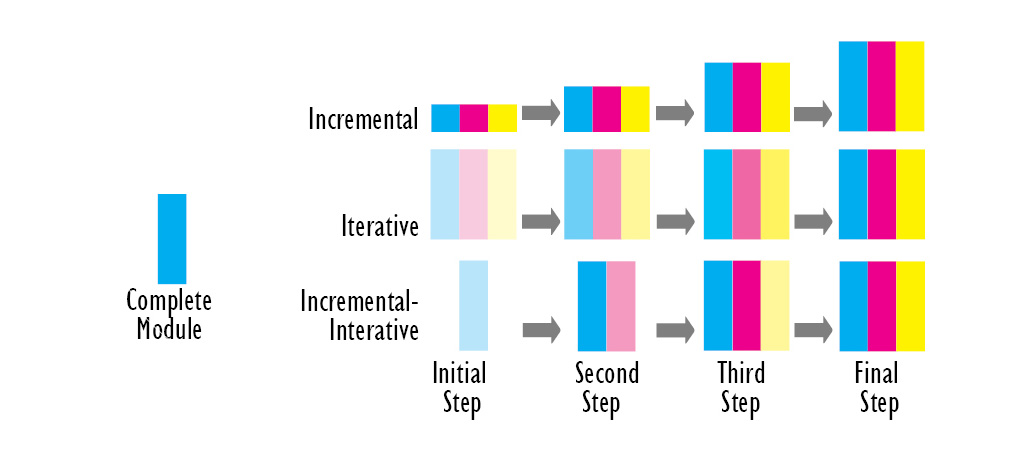
\includegraphics[scale=1.3]{img/Incremental-Interative-Design-Approach.jpg}
\caption{Incremental Iterative Development}
\label{Agile}
\end{figure}

\par Iterative and Incremental development is a process that combines the iterative design method with the incremental build model. The combination is of long standing  and has been widely suggested for large development efforts. This Agile method approach to Software Development is modeled around gradually increasing the features of a program and a cyclical release and upgrade pattern. The process usually begins with planning and continues through iterative cycles and the addition of features finishing with the development of a completed program of application at the end of each of these iterative cycles. Below we'll explain each of these individually:
\begin{itemize}
    \item Iterative: The incremental method divides the software development process into tiny, manageable chunks called increments.Each increment builds on the previous edition, allowing for gradual progress. 
    \item Incremental: Iterative software development refers to the process of repeating software development tasks in loops known as iterations. For each iteration, a new version of the program is created before the best product is found. 
\end{itemize}

This method of development was the main approach that we followed for the first semester of the year. We would meet weekly, discuss what needed to be done, and try to achieve it before the next meeting. On the 1st of December, our teammate, Anton Golubev, informed us that he would be leaving the course and deferring the year. This was a shock to both of us and meant that our workforce dropped by a third. \par
This drastic change in our design and development led us to try another approach to our development method. We decided to use Pair Programming, as we were now strictly Front End and Back End developers. As Cathal had more knowledge of the Back End internals, with less knowledge of the Front End, and Nathan being Vice Versa, this method allowed us to work more efficiently together with each others helping hand. \par
\begin{itemize}
    \item Pair Programming: This is an agile software development method that involves two programmers working at the same station. One developer writes the code while the other coaches the programmer, and reviews and assists in the writing of the code.
\end{itemize}
\par Our creation process and individual comprehension of the programs improved dramatically after we switched to pair programming.
It reduced the amount of time wasted due to small errors and sped up the production process on both ends. It helped each end of the application to understand what the other required in order to work properly.  \par
We returned to using the Iterative and Incremental development approach to correct individual bugs and features within the different development environments until the bulk of the development was completed. 

\section{Validation testing}
This part of the methodology will be dedicated to the Validation testing of our project. This is the method of testing software during the development process or at the end of the development process to see whether it meets those specifications. \par
Validation testing guarantees that the product meets the client's, or in our case, our project's, requirements. It can also be described as demonstrating that the product performs as expected when used in the designated environment. In short it is designed to answer if the product meets the requirements specified.\par
Testing is an integral aspect of a software project's life cycle, and it contributes to the overall consistency and reliability of the code in the project. The main form of testing that we incorporated into the project was white box testing. 
\begin{itemize}
    \item White Box Testing: In this form of testing, the tester has complete knowledge of the software's architecture, implementation, and internal structure. 
\end{itemize}
\par We used this method of testing by means of Postman and Robo 3T. We would send GET/POST/DELETE requests from Postman, while our Spring Boot application and Docker was running, and check for the exact out puts in Robo 3T by checking the MongoDB.

\section{Use of GitHub}
GitHub was essential to us during the development phase of the project. The use of GitHub in our development not only allowed us to save and exchange code with ease, but it can also double as a version control manager. We had all used GitHub for personal and academic projects, so we were all very familiar with the hosting service already. \par
Creating a GitHub repository was the first step in our development. Cathal created it and later added Nathan, Anton and Martin as collaborators to the repository. We tried to ensure that we never committed broken code to the repository so that there was always a working version of the application stored there. This method became essential to us at numerous times during the development. There were occasions when each of us had broken our own code beyond repair, and it was much more effective to simply clone the repo to the last working version than to try to reverse the code. 

\section{Criteria}
\subsection{React}
React is an open-source, front end, JavaScript library for building user interfaces or UI components. It is maintained by Facebook and a community of individual developers and companies \cite{React}. We decided to use this for our Front End as it aesthetically pleasing and once saved, the page will update automatically allowing for a quicker and easier development process.

\subsection{Node js}
Node JS is an asynchronous event-driven platform built on Chrome's JavaScript runtime that allows easy building of efficient, scalable network applications. NPM, or Node Package Manager is the Node JavaScript platform's package manager. It puts modules in place so that node can find them and intelligently manages dependency conflicts \cite{NodsJS}. Hundreds of thousands of JavaScript developers use it every day because it's battle-tested and remarkably versatile.

\subsection{Express}
Express is a Node.js web application framework that offers a comprehensive set of features for web applications. Express adds a thin layer of basic web application functionality without masking any of Node JS's known features \cite{ExpressJS}. When utilized correctly, express offers data to be fetched from the server and displayed to the client with ease and offers high scalability as well as exemplary security. It is well constructed and documented, making implementation quite an easy and fast process.

\subsection{Java}
Java is a class-based, object-orientated programming language that is designed to have as few implementation dependencies as possible \cite{Java}. This is the language that our Back End API, wrote in the Spring Boot framework, relies on. As we chose our API framework in Spring Boot first, we subsequently had to develop it in in Java. This language is one that Cathal has been programming for 6 years in, so as he focused on the Back End Development this was an ideal language to choose.

\subsection{Spring Boot}
Spring Boot is an open Source Java-Based framework used to create a micro Service. We used this framework to create and store collections in our Mongo Database. Spring Boot is developed by the team at Pivotal, it was designed to simplify the development of a new Spring application. The framework takes an opinionated approach to configuration, freeing developers from the need to define boilerplate configuration. Spring boot provides a good platform for Java developers to develop a stand-alone and production-grade spring application \cite{Javapoint}.

\subsection{MongoDB}
MongoDB is a document database, which means it stores data in JSON-like documents \cite{Mongo}. When it came to a decision as to what to use for our database, we had two main choices, MySQL and MongoDB. We both had more experience with MySQL and decided to use a Mongo Database instead to expand our knowledge and experience with more types of technologies.

\subsection{Docker}
Docker is a tool designed to make it easier to create, deploy, and run applications by using containers. Containers allow the developer to package up an application with all of the parts it needs, such as libraries and other dependencies, and deploy it as one package \cite{Docker}. This was an ideal platform to store our Mongo Database on, and to package our Front End and Back End for deployment on AWS.

\subsection{Robo 3T}
Robo 3T (formerly Robomongo) is a graphical user interface (GUI) for MongoDB hosting deployments that allows users to interact with their data through visual indicators instead of a text-based interface. We decided on using this to confirm objects being added to our collections as we found the visual indicator to be very pleasing when in comparison to a Command line interface that we would normally use when deploying to a Mongo Database.

\subsection{Postman}
Postman is an API client that makes it easy for developers to create, share, test and document APIs. This is done by allowing users to create and save complex HTTP/s requests, as well as read their responses. This allows users to automate manual tests and integrate them into their CI/CD pipeline to ensure that ant code changes wont break the API in production \cite{PostMan}. \par
This allowed us to test our Back End development was working and could POST and GET API calls without a Front End Environment being connected.

\subsection{AWS}
Amazon Web Services (AWS) is a secure cloud service platform, offering compute power, database storage, content delivery and other functionality to help businesses scale and grow \cite{AWS}. In short, AWS allows the user to run a web application server in the cloud. This is the technology that we decided best suited our needs for deploying the application onto a live server.

\subsection{IntelliJ}
IntelliJ IDEA is an integrated development environment written in Java for developing computer software. It is developed by JetBrains, and is available as a community licensed edition and as a commercial edition. This is the IDE we chose for developing our Java code as it is a visually pleasing and organised IDE \cite{IntelliJ}. Most of our Java modules required us to use Eclipse, so this was also a nice method of keeping our Final Year Project separate from our other Java code.

\subsection{Visual Studio Code}
Visual Studio Code is a freeware source-code editor made by Microsoft for Windows, Linux and mac OS. It has supported features for debugging, syntax highlighting, intelligent code completion, snippets, code refactoring and embedded GIT. This IDE is ideal for development of JavaScript as it provides a clear and concise UI for the developer.

\subsection{GitHub}
GitHub Inc is an internet hosting company that specializes in Git-based software creation and version control. It includes git's distributed version control and source code management features as well as its own.  We have been using this platform to store our projects since second year of college, so it was an ideal platform for us to use again, while ensuring we both had the most up to date version of our code.

\subsection{Jira}
Jira is a proprietary issue tracking product developed by Atlassian that allows bug tracking and agile project management. This software allows users to create weekly sprints with goals and deadlines to be achieved \cite{Jira}. We found this to be an ideal methodology for keeping us both knowledgeable of what is to be accomplished next and what needs to be completed.

\subsection{Discord}
Discord is a community-building tool that combines VoIP, instant messaging, and digital delivery.
In private conversations, users communicate using voice calls, video calls, text messages, media, and files. We used this platform to communicate live when we were both in development. We also used it to exchange texts, code and images with each other through a Discord Server we created.

\subsection{Facebook Messenger}
Facebook Messenger is an American messaging app and platform developed by Facebook inc. This is another service that allows for instant massaging between users. This was our main source of communicating with each other for organisation as it has been our main form of communicating since we were in first year.

\subsection{Microsoft Teams}
Microsoft Teams is a proprietary business communication platform developed by Microsoft. Teams offers work space chat and videoconferencing, file storage and application integration. When Covid-19 first affected us, GMIT switched to using Microsoft Teams for their main form of lecturing and live meetings. We used this platform weekly to have meeting with our supervisor and to communicate with them for advice.

% Check out the nice graphs in Figure \ref{tikz:graphs}, and the nice diagram in Figure \ref{tikz:mydiagram}.

% \begin{figure}
%   \centering
%   \begin{tikzpicture}
%   \begin{scope}[every node/.style={circle,thick,draw}]
%   \node (a) at (0,2) {a};
%   \node (b) at (2,2) {b};
%   \node (c) at (2,0) {c};
%   \node (d) at (0,0) {d};
%   \end{scope}
%   \begin{scope}[every edge/.style={draw=black,thick}]
%   \path (a) edge (b);
%   \path (b) edge (c);
%   \path (b) edge (d);
%   \path (c) edge (d);
%   \end{scope}
%   \node () at (1,-1) {$G_1$};
%   \end{tikzpicture}
%   \hspace{1.5cm}
%   \begin{tikzpicture}
%   \begin{scope}[every node/.style={circle,thick,draw}]
%   \node (1) at (0,2) {a};
%   \node (2) at (2,2) {b};
%   \node (3) at (2,0) {c};
%   \node (4) at (0,0) {d};
%   \end{scope}
%   \begin{scope}[every edge/.style={draw=black,thick}]
%   \path (1) edge (2);
%   \path (1) edge (3);
%   \path (1) edge (4);
%   \path (3) edge (4);
%   \end{scope}
%   \node () at (1,-1) {$G_2$};
%   \end{tikzpicture}
%   \caption{Nice pictures}
%   \label{tikz:graphs}
% \end{figure}


% \begin{figure}
%   \centering
%   \begin{tikzpicture}[node distance=6cm]
%   \node (a) [rect] {A Big Blue Block};
%   \node (b) [oval, right of=a] {And His Oval Friend};
%   \draw [line] (a) -- (b);
%   \end{tikzpicture}
%   \caption{Nice pictures}
%   \label{tikz:graphs}
% \end{figure}


\chapter{Technology Review}
 When we decided that we would be developing a CRUD application our first step was to decide upon what technologies we would be using to develop and test the application. This section will be split into four main focus points; The technology used in the Front End of the application, the technology used in the Back End of the application, the technology used for development, and the technology that is used to organise the development process of the application.
\begin{itemize}
\item The Front End: the technologies that were used in the Front End development were React, Node.js and Express.
\item The Back End: the technologies that were used in the Back End development were Spring Boot, MongoDB, Docker, Robo 3T, Postman and AWS.
\item This section will cover the technology used for the development process, mainly the Integrated Development Environments, IntelliJ and Visual Studio Code.
\item Lastly is the technology used in the organisation of the project development: GitHub, Jira, Discord and Microsoft Teams.
\end{itemize}

\section{Front End Technology}
\subsection{React}
The front end for this website was coded up using the React framework. We had only used React once before, in 3rd year, when we created a MERN (MongoDB, Express, React, Node) web application. Although one module during semester wasn't too much time, it was evident during this period that as well as being well documented and relatively user friendly, React is a very advanced framework.

\begin{figure}[th]
\renewcommand\thefigure{3.1}
\centering

\includegraphics[scale = .2]{img/reactImage.jpeg}
\caption{React logo}
\label{React}
\end{figure}

\subsubsection{Why React?}
There was a wide range of technical problems which was faced in web development.A large number of these problems were solved when Facebook came out with react and it has been constantly improving since its release in May 2013. \cite{IntroductionReact}React was brought out to solve complex user interface problems and utilizes a philosophy first thought up by Eric Raymond in 2003.

\begin{quote}
\emph{The only way to write complex software that won't fall on its face is to hold global complexity down - to build it out of simple parts connected by well defined interfaces - so that most problems are local and you can have some hope of upgrading a part without braking the whole - Eric S. Raymond} \cite{ArtOfUnix}
\end{quote}

\cite{IntroductionReact}React allows data to be displayed on wide scale user interfaces with relative ease. While most frameworks adopt a model, view, controller architecture, it would not be entirely accurate to place React under this category as React focuses more on the "view" as opposed to the model and controller. \par
React has a range of libraries which can be imported to add functionality to the framework. An example of a library which was used is axios, which is a library that aids the sending of http requests to external resources. \cite{Axios}Axios, as well as many of the other React libraries is well documented and has plenty resources out there to aid development.

\subsection{Nods.js}
We used Node JS because it provides all of the benefits of \cite{fullStackJS}full stack JS development. These include

\begin{itemize}
    \item Improved overall efficiency and productivity
    \item Better speed and performance
    \item Wide range of free tools
\end{itemize}

Due to its asynchronous, single-threaded nature, it works very well with React's responsive web pages and this was very useful during development as it minimised the time to wait between adding a feature and seeing if that feature worked since the website updated in what was pretty much real time. Big companies such as PayPal use NodeJS as apposed to something like Java and it's known to allow faster serving of web pages as well as reducing the time it takes to develop server-side software.\cite{PaypalNodeJS}\par
Node makes it very easy to handle all the packages that are required to run the application. It performs a lot of processes with efficiency in the background and provides very user friendly error messages whenever any problems arise during the installation of packages or when running the server. Node removes a lot of the heavy work involved in getting a website to function correctly, and it works extremely well when coupled with React.

\subsection{Express}
Express has some \href{https://expressjs.com/en/5x/api.html}{good quality documentation}. And although we only coded a tiny portion of this website using express, it was well documented, making it easy to find what we were looking for and implement it correctly. As express state that they are a \emph{"Fast, unopinionated, minimalist web framework for node."} Express provides robust routing, focuses on high performance, has great test coverage, provides HTTP helpers for things like caching and redirection.\cite{ExpressRM} Express also provides an executable which provides simple and quick generation of applications. 

\subsubsection{express.json} 
Json is a built-in middleware function in Express. Express.json parses requests received with JSON payloads and it is based on body-parser, which parses incoming request bodies in a middleware. 

\subsubsection{express.router}
A router Object behaves like middleware in that its sole purpose is performing routing and middleware functions. The express router offers a wide range of methods which can be used to acquire all sorts of routing functionality that enable the top level express object to essential operate as a router. Express router can be used with Nodemailer to send emails with fast routing.

\subsubsection{Nodemailer}
Nodemailer is a NodeJS module that makes sending emails much easier than one would expect. First released in 2010, at a time where sending email messages was a difficult task, it has now evolved to be the preferred solution for the majority of NodeJS users.
The Nodemailer team have a strong focus on security and integrity, which was the main reason why we saw it fit to be our email sending module of choice.

\subsection{Other technologies considered}
We also considered Angular for the back end framework since we also used Angular for a semester. However, along with Nathan's personal preference of React, its virtual DOM makes it perform much better than Angular. Also, React is the more popular framework and this wider community means more documentation and more activity on forums such as \underline{\href{https://stackoverflow.com}{StackOverflow}}. React goes well with Spring Boot and MongoDB, which was another leading factor in deciding what back end technology to use. \par

\section{Back End Technology}

\subsection{Java}
\begin{figure}[th]
\renewcommand\thefigure{3.2}
\centering

\includegraphics[scale = 0.31]{img/java-logo-1.png}
\caption{Java logo}
\label{Java}
\end{figure}
\newpage

The main coding language used on the Back End Development of the project is Java. Java was originally developed by James Gosling at Sun Micro systems (Later to be acquired by Oracle) and released in 1995 as a core component of Sun Micro systems' Java platform. Java is a general-purpose programming language intended to let application developers write once, run anywhere(WORA), meaning that compiled Java code can run on all platforms that support Java without the need of recompilation \cite{Java}. \par
This was the main reason in our choosing of the language for an application in which we intended to deploy, allowing us to not have to worry about errors once the program executed locally without any compilation errors. This is also a language in which we both had many years of experience in allowing us to commit the time we had gained by already knowing the language for our development, into other technologies we hadn't used such as AWS or MongoDB.

\subsection{Spring Boot}
Spring Boot Auto Configuration automatically configures the Spring Boot Application based on the JAR dependencies added in the project. For example with this application when we are using the Mongo Database, we don't need to configure a database connection, the Spring Boot auto-configures an in-memory database. To do this though we must add the @EnableAutoConfiguration annotation to the main class file. Then the Spring Boot application will be automatically configured.\par
Spring Boot application scans all the beans and package declarations when the application initializes. the @ComponsnentScan annotation must be added for the class file to scan the components added to the project. \par
The class that contains the @SpringBootApplication and the main method is the entry point of the spring boot application. This class must have the main method to run the Spring Boot applicaton. The @SpringBootApplication annotation includes the Auto-configuration, Component Scan and the Spring Boot Configuaration. Since the @SpringBootApplication annotation has been added to the main class we do not need to add the @EnableAutoConfiguration, @ComponentScan and the @SpringBootConfiguration annotations. The @SpringBootApplication annotation includes all other annotations. \par
See the following code for a better understanding:
\begin{minted}{java}
import org.springframework.boot.SpringApplication;
import org.springframework.boot.autoconfigure.SpringBootApplication;

@SpringBootApplication
public class FyPprojectApplication {

	public static void main(String[] args) {

		SpringApplication.run(FyPprojectApplication.class, args);
	}

}
\end{minted}
Spring Boot's use of these Auto-configuration allowed us to streamline our development of the Back End Environment of the project. Simply by adding dependencies into our pom file of the Spring Boot application, our program will auto-configure it upon compile time. \par
\begin{minted}{java}
<dependency>
	<groupId>org.springframework.boot</groupId>
	<artifactId>spring-boot-starter-data-mongodb</artifactId>
</dependency
\end{minted}
\cite{TutorialsPoint}

\subsection{MongoDB}
\begin{figure}[th]
\renewcommand\thefigure{3.3}
\centering

\includegraphics[scale = 0.5]{img/MongoDB-logo.png}
\caption{MongoDB logo}
\label{MongoDB}
\end{figure}

MongoDB is the leading modern, general purpose database platform, designed to unleash the power of software and data for developers and the applications they build. Its built upon the document model, a fundamentally different model than traditional relational databases. \par
In real world applications it is common place for the data for a single object, like a patient or a user, to spread out among dozens of tables. This adds a massive amount of complexity to the application. This can add a number of downsides to the application:
\begin{itemize}
\item It can make the maintenance of the application hard to understand
\item Secondly it can make adding features harder as there is more to account for
\item Lastly pulling data from so many areas is inefficient and the applications need to have code to deal with this
\end{itemize}
\par MongoDB takes an entirely different approach, data is stored in records called documents and just like real physical records, documents can house multiple phone numbers, addresses and more and can be right next to another document that only has one address and no phone number. Records aren't restricted to having the same number of columns. These documents allow us to store data in a way that is easy for the computer to process and natural for humans to read. This allowed us to no longer have to make our application accommodate the needs of the database. MongoDB accommodates us, to allow us to store our data in a more natural way. This allowed us to add new data to each collection without having to worry about breaking previous data. \par

\subsection{Docker}
\begin{figure}[th]
\renewcommand\thefigure{3.4}
\centering

\includegraphics[scale=0.2]{img/docker-logo.png}
\caption{Docker logo}
\label{Docker}
\end{figure}

Docker is a Software Development platform with aspects of a virtualisation technology that makes it easy for developers to develop and deploy applications inside neatly packaged virtual container environments \cite{Docker}. This means that Docker allows applications to run the same no matter where they are or what type of machine they are running on. Docker containers can be deployed to any machine without any compatibility issues so that our software stays system agnostic making the software simpler to use, less work to develop and easy to maintain and deploy. \par
These containers running on the computer or server act as miniature micro heaters, each with their own specific job, operating system,isolated CPU processes, memory and network resources. Because of this these containers can be easily added, removed, stopped and started without affecting the run time machine. Containers usually run one specific task, in our case that is the Mongo Database, the React application and the Spring Boot application. These containers are then networked together and potentially scaled. A developer can access the Docker Hub and pull a pre-configured container designed for a specific task from the Hub and integrate it into their own environment. We deiced to make these containers ourselves to gain a better understanding and knowledge of our containers and to ensure that the containers were not executing any unneeded or redundant features.

\subsection{Robo 3T}
\begin{figure}[th]
\renewcommand\thefigure{3.5}
\centering

\includegraphics[scale=0.6]{img/robo-logo.png}
\caption{Robo logo}
\label{Robo}
\end{figure}

Robo 3T is effectively a MongoDB manager. We used Robo 3T to check the Mongo database without having to use a Command Line. This allowed us to visualise our database in a more innovative way. It can be used on multiple OS's including Windows, Linux and MAC. Once Robo 3T has been loaded, it will open up a GUI asking for the user to connect to. \par
\begin{figure}[th]
\renewcommand\thefigure{3.6}
\centering
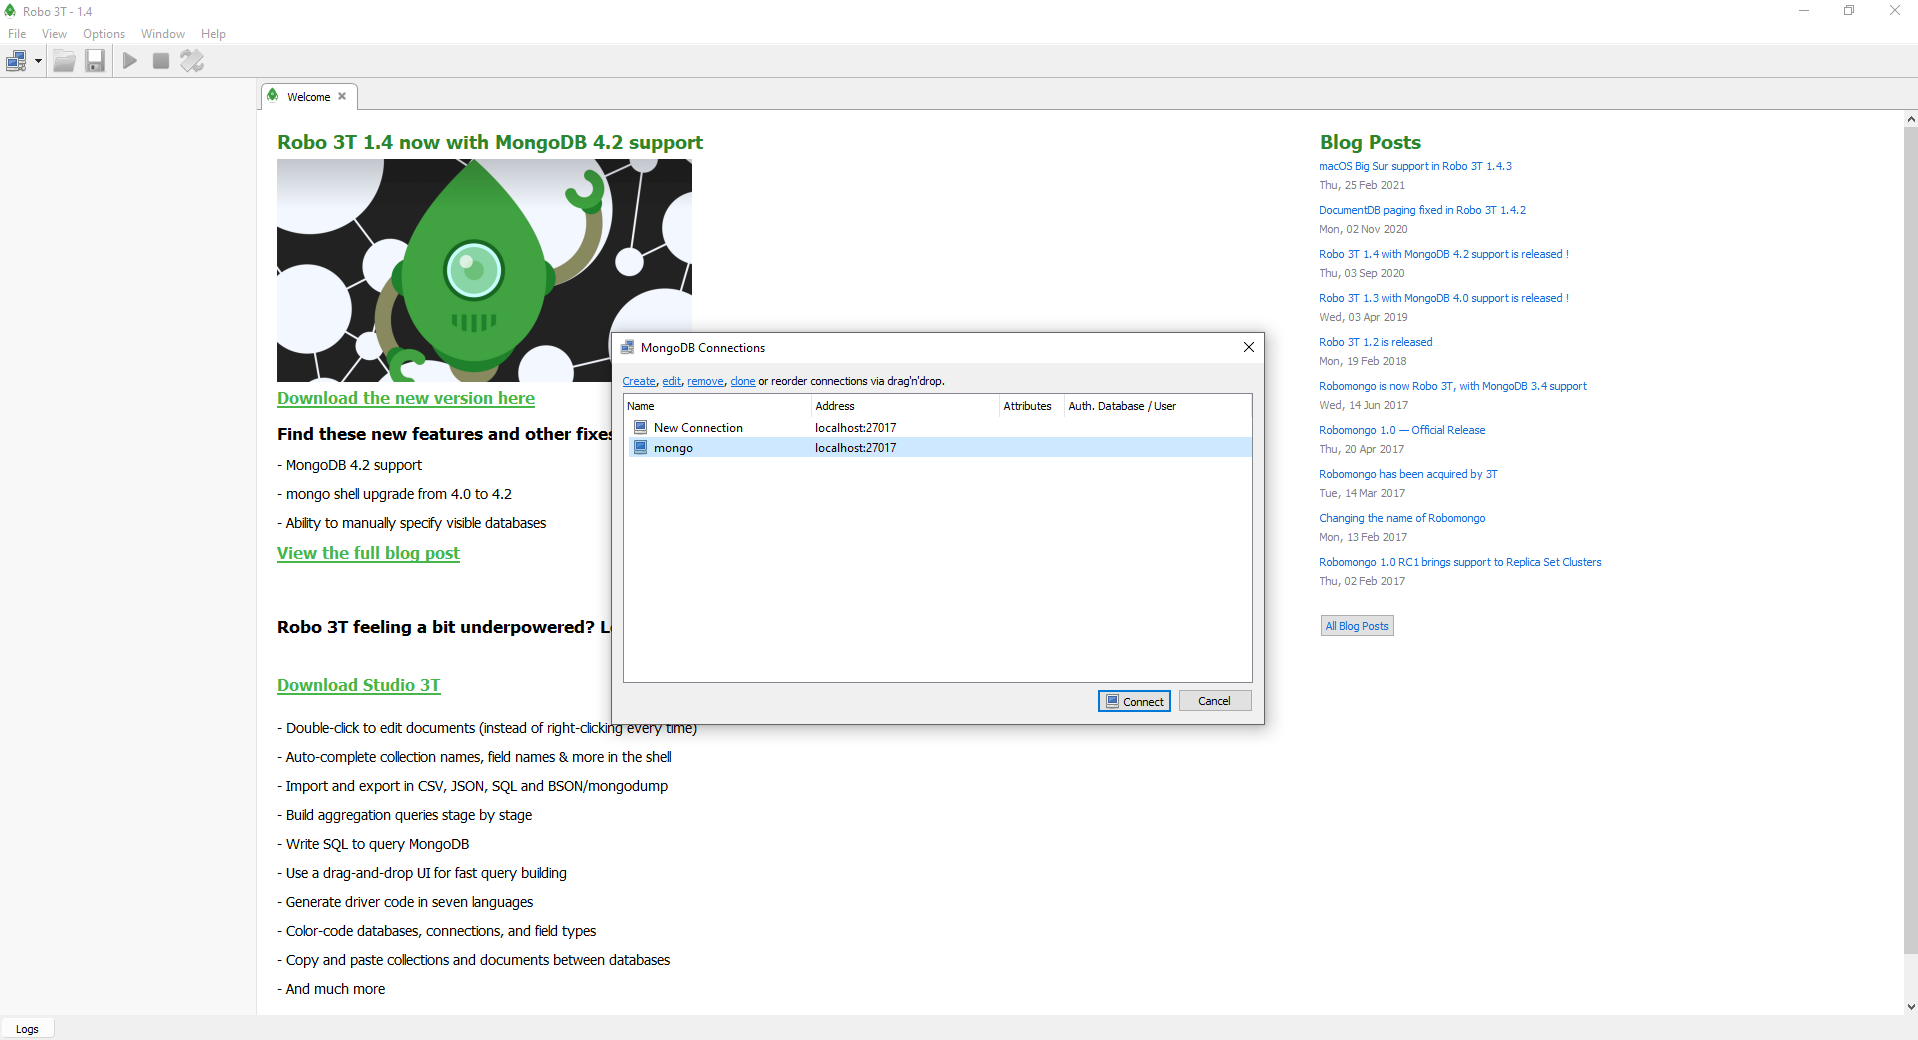
\includegraphics[scale=0.3]{img/robo-connect.PNG}
\caption{Robo software}
\label{RoboSoftware}
\end{figure}

From here the user can select one of the connections, and providing that a MongoDB database is currently running on one of the machines ports, Robo 3T will connect to it displaying contents similar to the following: \par
\begin{figure}[th]
\renewcommand\thefigure{3.7}
\centering
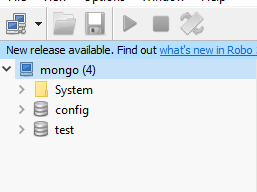
\includegraphics[]{{img/robo-contents.PNG}}
\caption{Robo content I}
\label{RoboContentI}
\end{figure}

The user can then select their MongoDB database, in this case it is test, and Robo 3T will display all of the collections within this database. \par
\begin{figure}[th]
\renewcommand\thefigure{3.8}
\centering
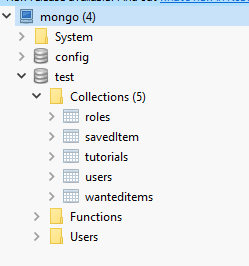
\includegraphics[]{{img/robo-collections.PNG}}
\caption{Robo content II}
\label{RoboContentII}
\end{figure}

The user can then select these collections and execute various commands that would normally be entered into a command line interface. \par
\begin{figure}[th]
\renewcommand\thefigure{3.9}
\centering
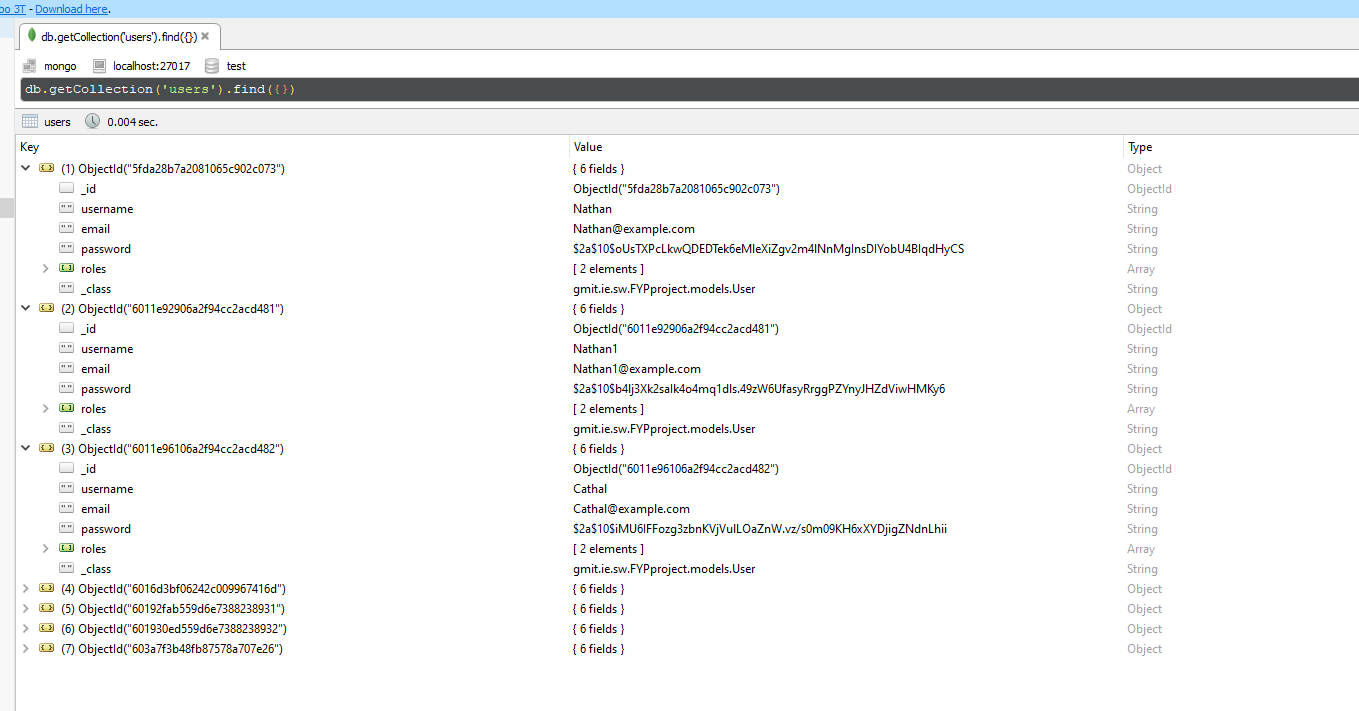
\includegraphics[scale=0.35]{{img/robo-users.PNG}}
\caption{Robo users}
\label{RoboUsers}
\end{figure}

As we can see above, Robo 3T executes these commands, this time it being: 
\begin{minted}{bash}
db.getCollection('users').find({})
\end{minted}
This can save many users the much needed time that would otherwise be lost in a CMD window trying to configure the requests and ensuring that their syntax is correct.

\subsection{Postman}
\begin{figure}[th]
\renewcommand\thefigure{3.10}
\centering

\includegraphics[scale=0.4]{{img/postman-inc-logo-vector.png}}
\caption{Postman logo}
\label{Postman}
\end{figure}

Postman is a modular API testing tool that integrates seamlessly into your CI/CD pipeline.Before connecting the API to the Front End React environment, we used Postman to send API requests to the Spring Boot application while it was live. Cathal was able to function and test his environment without the need for Nathan to attach it to the Front End as a result of this. \par
Postman is incredibly easy to set up on ones machine. Simply download the application from the website and its ready to go. Postman is a tab based application, meaning that every time you want to test a new request function, we recommend you open a new tab. From here you're presented with something similar to this: \par
\begin{figure}[bh]
\renewcommand\thefigure{3.11}
\centering
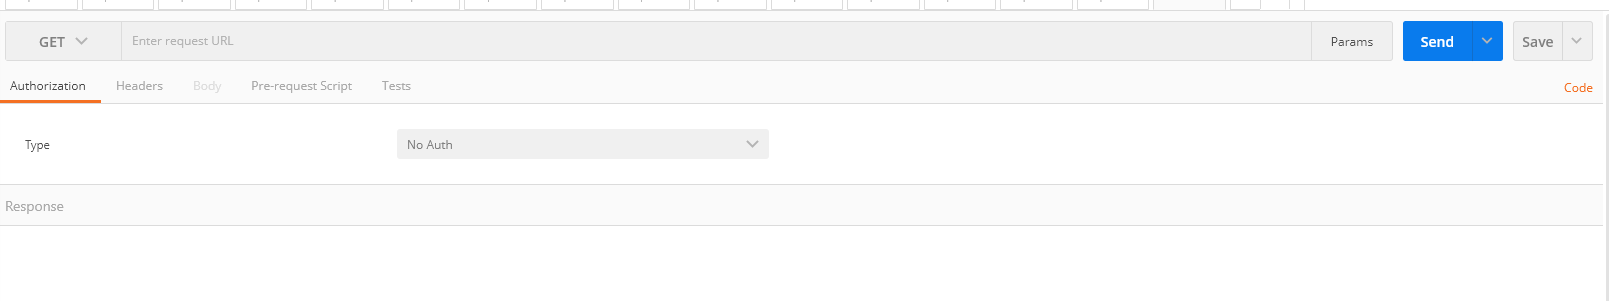
\includegraphics[scale=0.3]{img/postman-tab.PNG}
\caption{Postman tab}
\label{PostmanTab}
\end{figure}

\par As you can see, the user can then select the type of request they mean to specify eg. GET/POST/PUT/DELETE. Then when they enter the specified URL, http://localhost:8081 for example, they can then select the body. This part of Postman is where the user decides what to enter. As MongoDB is a document based database structure, we send raw JSON data with our requests. \par

\begin{figure}[bh]
\renewcommand\thefigure{3.12}
\centering
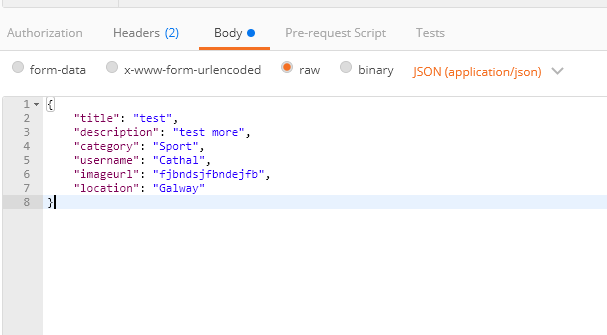
\includegraphics[scale = 0.8]{img/postman-JSON.PNG}
\caption{Postman body}
\label{PostmanBody}
\end{figure}

Then when the user clicks the "send" button, they will get a response specifying if the request was successful of if there was an error in the request. This was an excellent method of testing and confirming that the API calls were functioning before ever having to connect it to the Front End Environment.

\subsection{AWS}

\begin{figure}[h]
\renewcommand\thefigure{3.13}
\centering

\includegraphics[scale = 0.3]{img/aws_logo_smile_1200x630.png}
\caption{AWS logo}
\label{AWSLogo}
\end{figure}

AWS, also known as Amazon Web Services, is one of the leaders in the cloud computer market. AWS was first introduced in 2002 as a means to provide tools and services to developers to incorporate features of Amazon.com into their website. Its first cloud servicing was introduced in 2006. Today, AWS offer a wide range of cloud services that span a wide array of domains. Due to this, the AWS service is now used by over 45\% of the global market. \par
AWS is a secure cloud platform that provides computing power, database, networking, content storage and much more. The platform also works on a pay-as-you-go model, meaning you only pay as long as your service is running. Some of the other advantages of AWS are:
\begin{itemize}
    \item Security: AWS provides a secure and durable platform that offers end-to-end privacy and security.
    \item Flexible: It allows users to select the OS, Language and Database and other services.
    \item Scalable: Depending on user requirements, application can be scaled up or down.
\end{itemize}
In our project, we use AWS to host the Back End environment, the Front End Environment and the MongoDB Database off of the Docker containers we built. This allowed us to host our website with ease and to deploy it in a matter of days.

\subsection{Other Technologies considered}
Our initial idea for the back end was to use a python based Flask framework. However, after many failed attempts at getting a functional Flask application working, we decided to move onto a Spring Boot application instead. This was mostly due to another module we were doing at the time, Emerging Technology. This module involves the use of coding in python with the Anaconda. Anaconda is a free and open-source scientific computing distribution for the Python and R programming languages that aims to make package management and deployment easier. But with the installation of Anaconda, the commands set by Flask, to create and run a new Flask application, cannot be executed properly. To avoid breaking our Anaconda for that module, we opted to use Spring Boot instead. 

\section{Development Technologies}

\subsection{IntelliJ}
This is the Integrated Development Environment that we used for our Back End Java Spring Boot API. IntelliJ has many supported features built into its system. This was the optimal IDE of choice for the Back End environment as, being wrote in Java, it is very Object Orientated based. IntelliJ analyzes the code, looking for connections between symbols across all project files and languages.\par
Using this information, it provides in depth coding assistance, quick navigation, clever error analysis and refactoring. This allows IntelliJ to auto complete many lines of code as the developer works. This is an excellent IDE for Java developers, and can save some much needed time. The smart completion ensures less errors in ones code as oppose to developing on an IDE like Eclipse. IntelliJ isn't tasking on your machine allowing for developers of all levels to create great Java code.

\subsection{Visual Studio Code}
Visual studio code was the IDE which we used to help us create all of the front end code. VS code offers really good IntelliSense code completion as well as intuitive code refactoring and some quality debugging tools. Visual studio code is the leading choice of freeware source-code editor for the majority of React developers as the layout and IntelliSense works works better with typescript files than any other open source IDE.

\section{Organisation Technology}

\subsection{GitHub}
\begin{figure}[h]
\renewcommand\thefigure{3.14}
\centering

\includegraphics[scale=0.6]{img/github-logo.jpg}
\caption{GitHub logo}
\label{GithubLogo}
\end{figure}

GitHub has a multitude of different features to vastly improve the development of a project of any level of difficulty. GitHub is an online framework that can be used to host a variety of different programming languages such as Java, C++ and Ruby. GitHub is a git repository hosting service and can be used for version control management. \par
GitHub also has many social network functionalities built into its framework. A user on GitHub can follow other users, view their repositories and their projects, search the entirety of public GitHub repositories and more. This was the main method of storing, updating and trading code with one another. If a compile error on one of our ends were to develop, we could always clone the most recent version of our project back onto our machines instead of spending hours trying to roll back to when our own versions last compiled properly. \par
Below we will list some basic commands that users can enter into a Command-Line Interface (cmd) to initialise and to push to a repository of their own.

\subsubsection{Git commands}
\begin{minted}{console}
# to initialise a repository inside the current directory
git init

# to add all of the existing contents inside the directory to the repository
git add .

# a commit is when a user pushes to the repository. The message "first commit" can be changed to the user's preference allowing them to explain what the commit consists of
git commit -m "first commit"

# this contains the URL of the repository the user is pushing to
git remote add origin https://github.com/username/FirstRepo.git 

# command to finalise push
git push -u origin master


# push an existing repository from the command line
git add .
git commit -m "Another commit"
git push

\end{minted}

\subsection{Jira}
\begin{figure}[h]
\renewcommand\thefigure{3.15}
\centering

\includegraphics[scale=0.4]{img/jira.png}
\caption{Jira logo}
\label{JiraLogo}
\end{figure}

Jira is an online web application that allows users to create and set sprints. Jira can also allow you to inform your team of the latest bugs and problem, and also of new features of what has been done. These bugs, tasks or features can be documented deeply allowing for everyone on the team to be in the know and completely aware of these updates to their project. \par
Jira was mostly used by us in creating sprints for us to work on for the week or weeks ahead. We would set up our tasks and set up the goals, and as they are completed, they can be moved over to the "done" section allowing everyone on the team to be aware of this development in the project. \par

\begin{figure}[h]
\renewcommand\thefigure{3.16}
\centering
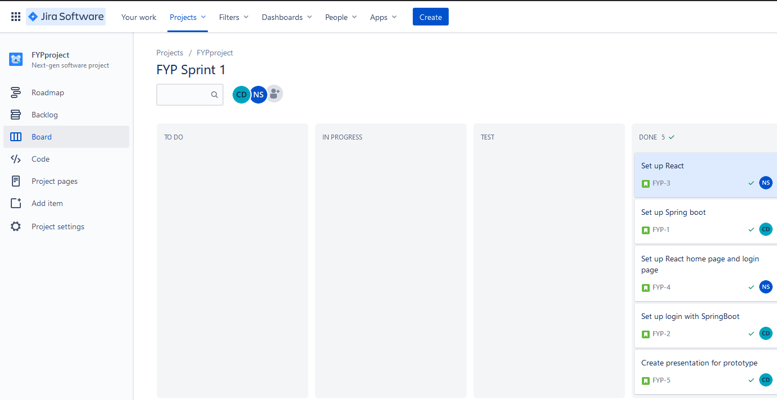
\includegraphics[scale=0.7]{img/jira-sprint.PNG}
\caption{Jira sprint}
\label{JiraSprint}
\end{figure}


\subsection{Discord}

\begin{figure}[hb]
\renewcommand\thefigure{3.17}
\centering

\includegraphics[scale=0.1]{img/discord-logo.jpg}
\caption{Discord}
\label{Discord}
\end{figure}
\par
The Discord application is an almost unbeatable means of communication between developers, especially in the world we live in today with the Covid-19 pandemic. Discord was essential in our development of this project, as when we were pair programming, refer to our methodology for more information on this, this was the platform we used to do so. Discord allows a user to share their screen, and all other members of the Discord call to view their screen in real time. Discord also has the feature of bots. These bots can do numerous functions. We created a Final Year Project Server on Discord for our development process. One of the bots included in this server was a bot called "Groovy". This bot allows users to enter commands into the text channels, requesting a song. The bot will automatically join the call and play the song in question. This was utilized a multitude of times to increase our moral and enthusiasm as we worked on the project. \par

\begin{figure}[h]
\renewcommand\thefigure{3.18}
\centering
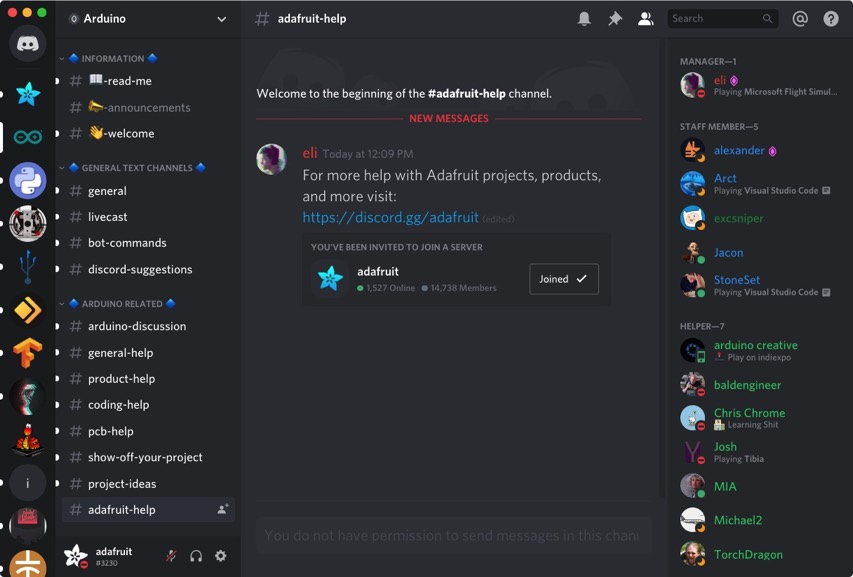
\includegraphics[scale=0.5]{img/server.jpg}
\caption{Discord Server}
\label{DiscordServer}
\end{figure}

\subsection{Facebook Messenger}
\begin{figure}[ht]
\renewcommand\thefigure{3.19}
\centering

\includegraphics[scale=0.3]{img/messenger.png}
\caption{Messenger logo}
\label{MessengerLogo}
\end{figure}

Facebook messenger was utilised by us as a form of communication when both of us were away from our machines. Since first year, this has been our main platform for communicating with one another so it was a natural choice for us to continue to use the platform for our planning and development. When one was working on the project and needed to get in touch with the other developer, we could utilize messenger's built in call feature. This will ring the receiver's phone the same as a normal telephone call, but doesn't require any credit, as unemployed students this was a great method for instantly getting in touch with one another.

\subsection{Microsoft Teams}

\begin{figure}[hb]
\renewcommand\thefigure{3.20}
\centering

\includegraphics[scale=0.4]{img/teams-728.jpg}
\caption{Microsoft Teams logo}
\label{TeamsLogo}
\end{figure}

In 2020 when the Covid-19 restrictions first came into place in Ireland, Galway-Mayo Institute of Technology switched to the Microsoft Teams platform to continue to do live lectures and labs. As the college decided to keep our course at home for the 2 semesters of our final year, Microsoft Teams was used very often with our modules for live labs and lectures. \par
This is the platform we used to communicate with our supervisor and to meet for our weekly meetings. GMIT linked our GMIT accounts with the Microsoft office, meaning we didn't even need to create an account for ourselves, and we were already connected to all of our lecturers and fellow students, saving us some much needed time. It has vast number of different features for users. It allows the user to do most of the same functions as Discord, but we used it for a more professional manner. We had a private chat between ourselves and Martin in which we could message each other and send in photos. This was used to communicate ideas and problems we came across in the development phase. \par

\begin{figure}[ht]
\renewcommand\thefigure{3.21}
\centering
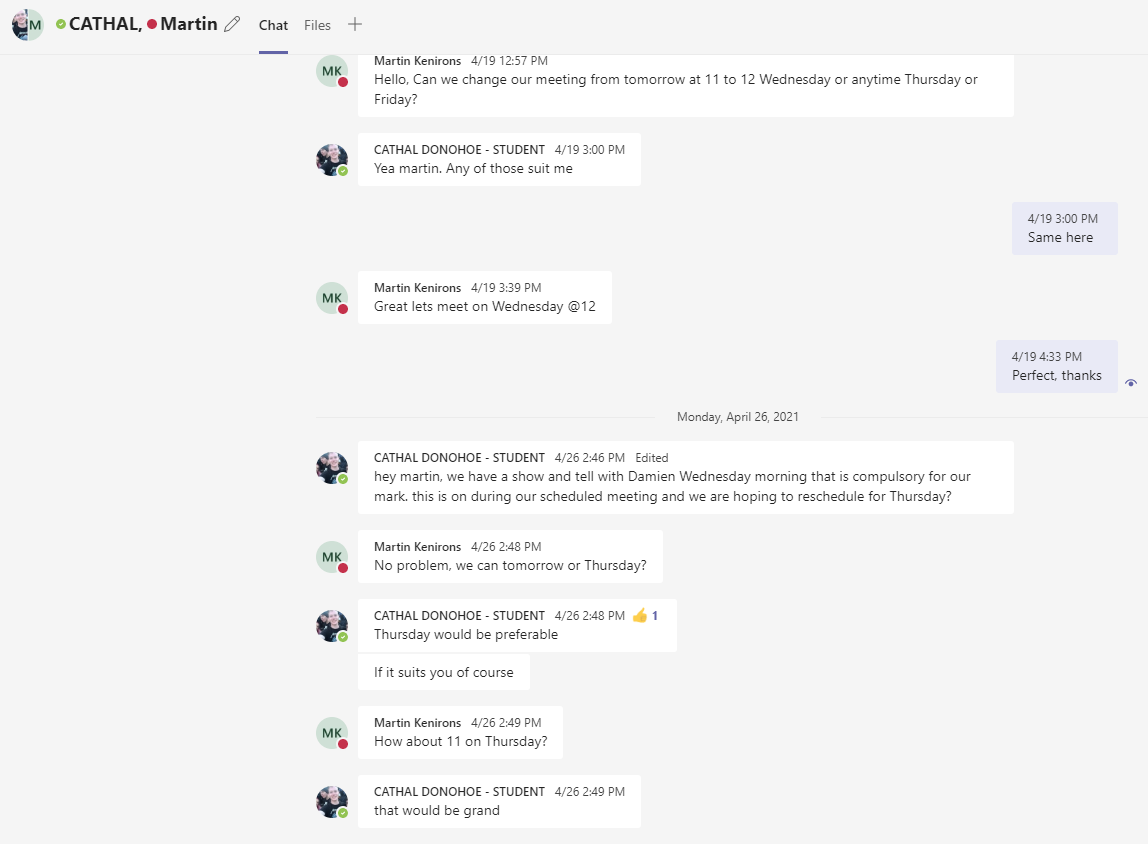
\includegraphics[scale=0.4]{img/teams.PNG}
\caption{Microsoft Teams chat}
\label{TeamsChat}
\end{figure}

Another important feature of Microsoft Teams is the ability to schedule meetings between multiple users for a specific Date and Time. This notifies all users invited that they have a scheduled meeting for this Time and Date. This was important in keeping us on top of our weekly meetings. As i stated above with the GMIT accounts and the Microsoft accounts being linked, if we logged into Windows built in Mail application with our GMIT accounts, the scheduled meetings automatically appear on the Windows calendar, further notifying the user of a meeting and ensuring ease of use and punctuality for that user.
\begin{figure}[ht]
\renewcommand\thefigure{3.22}
\centering
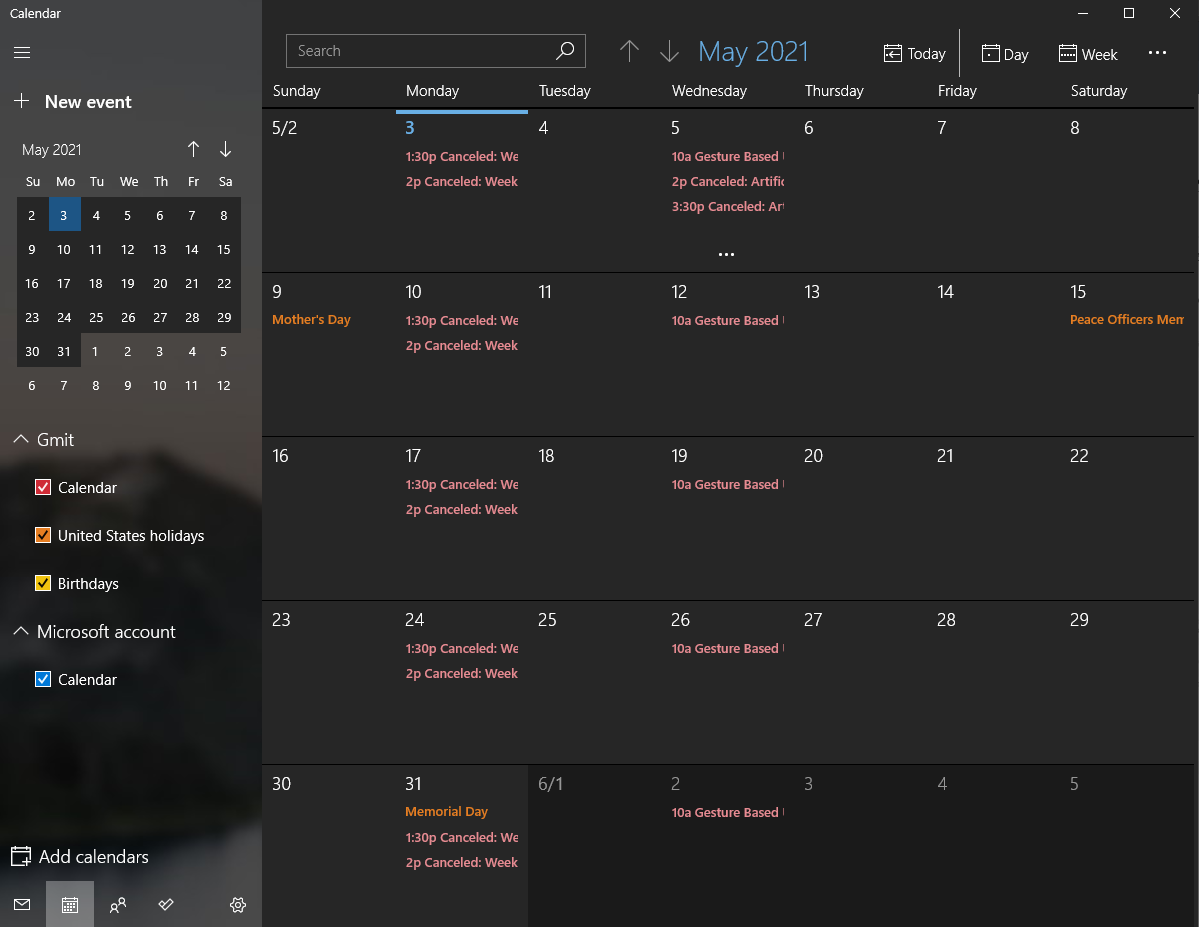
\includegraphics[scale=0.4]{img/Caledar.PNG}
\caption{Microsoft Teams calendar}
\label{TeamsCalendar}
\end{figure}


\begin{figure}[ht]
\renewcommand\thefigure{3.23}
\centering
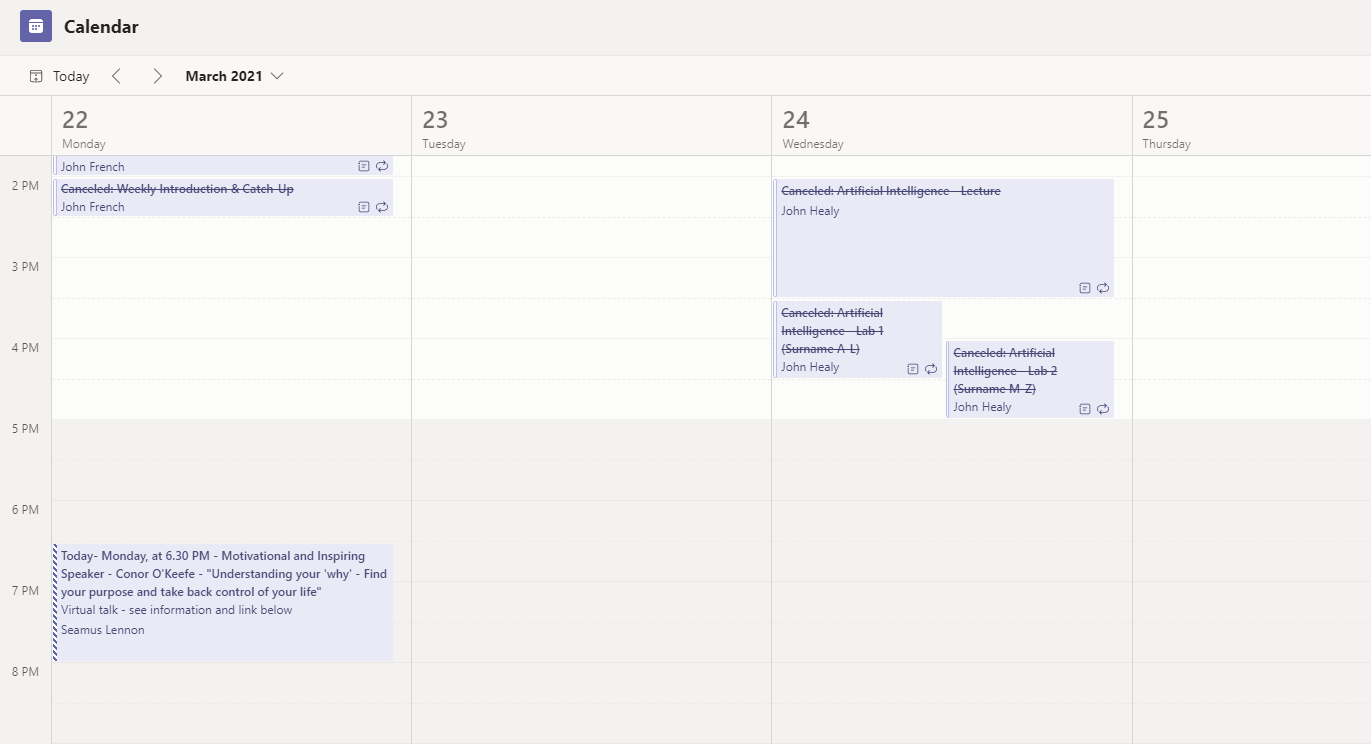
\includegraphics[scale=0.4]{img/TCalendar.PNG}
\caption{In Teams scheduled meetings}
\label{TeamsMeetings}
\end{figure}


\chapter{System Design}
%Provide a detailed explanation of the overall system
%architecture. The HOW of the project.
%– System designed should be informed by the technology review, i.e.
%you applied the knowledge that you learned doing the research…
%– Standards-based where possible. How are components coupled?
% – Cloud hosted – IaaS / PaaS / Sa.
% Use diagrams to augment an explanation of the architecture
%used.
%– Provide a comprehensive overview of the different components of
%the system and how they work together.
%– UML class, sequence and interaction diagrams.
%– Course and fine grain.
%– Use screen shots of forms or other UI components.
%q Page count range difficult to state as varies significantly
%between projects.
%As many pages as needed
This application is a React application that uses a Spring Boot API to communicate fetch and get requests from a MongoDB. The front end of this website is set up with React so that it is a single page application. These kind of websites offer a nice boost in performance, as all of the HTML, CSS and JavaScript is loaded as soon as the website is loaded. Single page applications perform efficient data caching which reduces loading times. SPA's also provide a much better overall experience for the user. \par
The Back End of this website is set up with Spring Boot. Spring Boot is a Spring module that provides the RAD (Rapid Application Development) feature to the Spring framework \cite{Javapoint}. Spring Boot is a project that uses the Spring Framework as its foundation.
It makes setting up, configuring, and running both easy and web-based applications simpler and quicker. This provides an overall much easier development time for the programmer. \par
Spring Boot communicates with the MongoDB Database through the Mongo Repositories set up within the Spring Boot API. The below image may provide more context for the reader:

\begin{figure}[ht]
\renewcommand\thefigure{4.1}
\centering
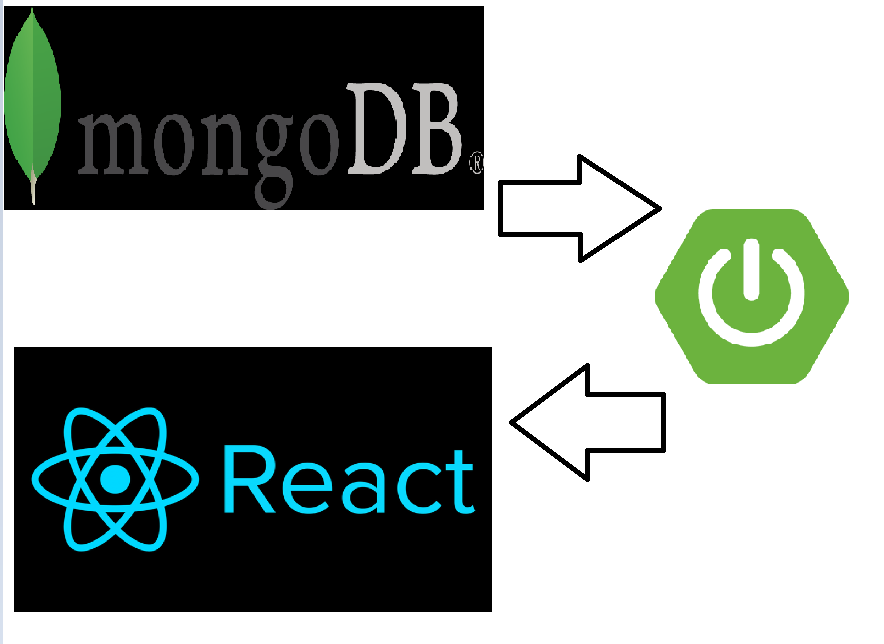
\includegraphics[scale=0.28]{img/architecture.png}
\caption{System architecture}
\label{SystemArch}
\end{figure}

\section{Overview of components}
\subsection{Front End}

\subsubsection{Starting out}
The \underline{\href{https://react-bootstrap.github.io/getting-started/introduction/}{ReactJS documentation}} explains how to use node and npm to build a new single-page application with the default template, which was an excellent starting point.
\begin{minted}[bgcolor=black,formatcom=\color{yellow}]{bash}
npx create-react-app my-app
cd my-app
\end{minted}

After building the app, which only took a few minutes, it is easy to to a point where it is accessible by running a node package manager command which runs a series of commands that enables the app to be viewed at the default url of \emph{localhost:3000}
\begin{minted}[bgcolor=black,formatcom=\color{yellow}]{bash}
npm start
\end{minted}

The next task was consuming the react-bootstrap package by following the \underline{\href{https://react-bootstrap.github.io/getting-started/introduction/}{React-bootstrap documentation}}. The node package manager was used to install the vanilla react-bootstrap package which allows us to customize the bootstrap Sass files. The package also removes the need to use a content delivery network for the stylesheet.
\begin{minted}[bgcolor=black,formatcom=\color{yellow}]{bash}
npm install react-bootstrap bootstrap
\end{minted}

\subsubsection{Sign Up}
Since the first semester was rather challenging for a number of reasons, our main goal was to have an example homepage along with working login and register pages prepared in time for our Christmas presentation. For this reason, sign up was the first front end component which was worked on. \par
The user can navigate to the sign up page by clicking on sign up in the navigation bar or by alternatively adding /signup to end of the URL. To sign up, users must provide a username, password and email address. 
\begin{figure}[ht]
\renewcommand\thefigure{4.2}
\centering
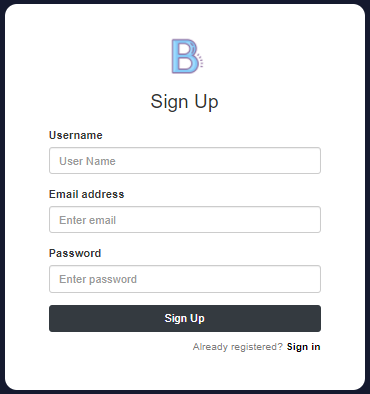
\includegraphics[scale=1]{img/fe_signup.png}
\caption{Sign up component}
\label{SignUp}
\end{figure}

Once signed up, the user is automatically logged in and redirected to the home. Since they're signed in, they're now permitted to access a number of additional features of the website such as adding an item or saving an item.  

\subsubsection{Login}
The login component is similar to the sign up component, except it only requires the user's username and password to be correct in order to log in and access the features which are blocked to anonymous users. 

Once logged in, there is a state change in the top navigation bar which changes the 'login' and 'sign up' options to the name of the user, which brings the user to their account page on click, as well as a logout option, which does exactly what it says on the tin.

\begin{minted}[fontsize=\footnotesize]{js}
 logout() {
        localStorage.clear();
        window.location.reload(false);
    }
{isLoggedIn && (
    <li className="nav-item">
    <Link className="nav-link" to={"/account"}>{myUser}</Link>
    </li>
)}
{isLoggedIn && (
    <li className="nav-item">
        <Link className="nav-link" onClick={() => 
        this.logout()}>{'Logout'}</Link>
    </li>
)}
{!isLoggedIn && (
    <li className="nav-item">
        <Link className="nav-link" to={"/login"}>Login</Link>
    </li>
)}
{!isLoggedIn && (
    <li className="nav-item">
        <Link className="nav-link" to={"/signup"}>Sign up</Link>
    </li>
)}
\end{minted}

\subsubsection{Homepage}
Coupled with the top nav bar, which is static and stays there no matter what page the user navigates to, the homepage also has a navigation bar on the side with links to the different pages they can access.

\begin{figure}[ht]
\renewcommand\thefigure{4.3}
\centering
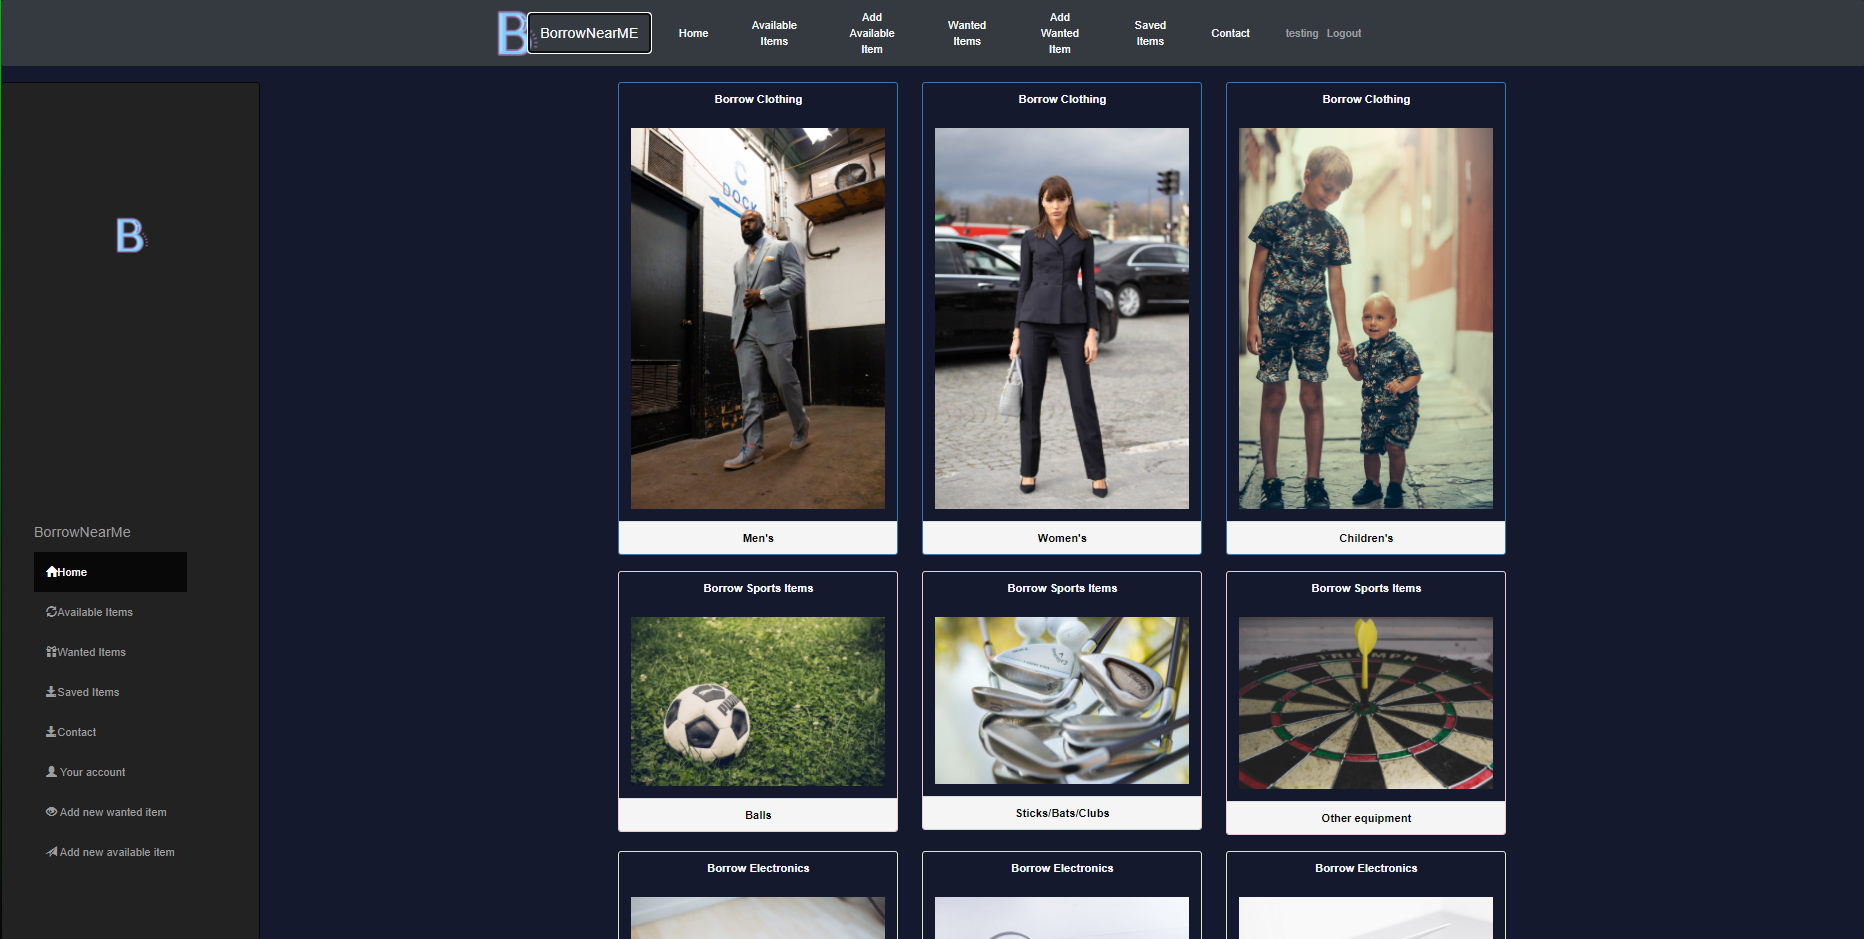
\includegraphics[scale=0.3]{img/fe_homepage.PNG}
\caption{Home page}
\label{HomePage}
\end{figure}

\par
The homepage also has a number of images which can be clicked to find available items which are filtered by the selected category.The homepage is quite intuitive and user friendly, making it easy for client's to find their way around the site.  

\subsubsection{View Items}
Users are able to view both the available and the wanted items which other users have listed on the website i.e. stored in the database. For the available items, the items are filtered only if the user accesses the available items by clicking on one of the categories on the homepage. Otherwise, all items will be displayed. The page that displays wanted items has a section at the top that allows the user to display all counties or filter by County.
\begin{minted}[fontsize=\footnotesize]{js}
{isFiltered == true && (
    <div key={index}>
        {items.category == filter && (
        <Card>
            <CardImg top width="100%" src={items.imageurl} alt="Card image cap" />
            <CardBody>
            <CardTitle tag="h4"><b>{items.title}</b></CardTitle>
            <CardSubtitle tag="h6" className="mb-2 text-muted">Category</CardSubtitle>
            <CardText>{items.category}</CardText>
            <CardSubtitle tag="h6" className="mb-2 text-muted">Description</CardSubtitle>
            <CardText>{items.description}.</CardText>
            <CardSubtitle tag="h6" className="mb-2 text-muted">Location</CardSubtitle>
            <CardText>{items.location}</CardText>
            <CardSubtitle tag="h6" className="mb-2 text-muted">Posted by</CardSubtitle>
            <CardText>{items.username}</CardText>
            <Link to={'/availableItems/' + items.id}
            className="btn btn-primary">See Item</Link>
            </CardBody>
        </Card>
        )}
    </div>
)}
\end{minted}

Each item has a button which can be clicked to display more information about that item. Once the user is signed in, they are able to send an email to the owner of the item if they wish. All they have to do is type their message to the user into the input box and once they click send, an email is sent to the owner of the item. This email is sent from our 'barter4tradenc@gmail.com' address and informs the item's owner of the name of the user interested in their item, the name of the item they're interested in and the message the user entered. There is also a button that allows the user to add an item to their list of saved items.
\newpage

\begin{figure}[ht]
\renewcommand\thefigure{4.3}
\centering
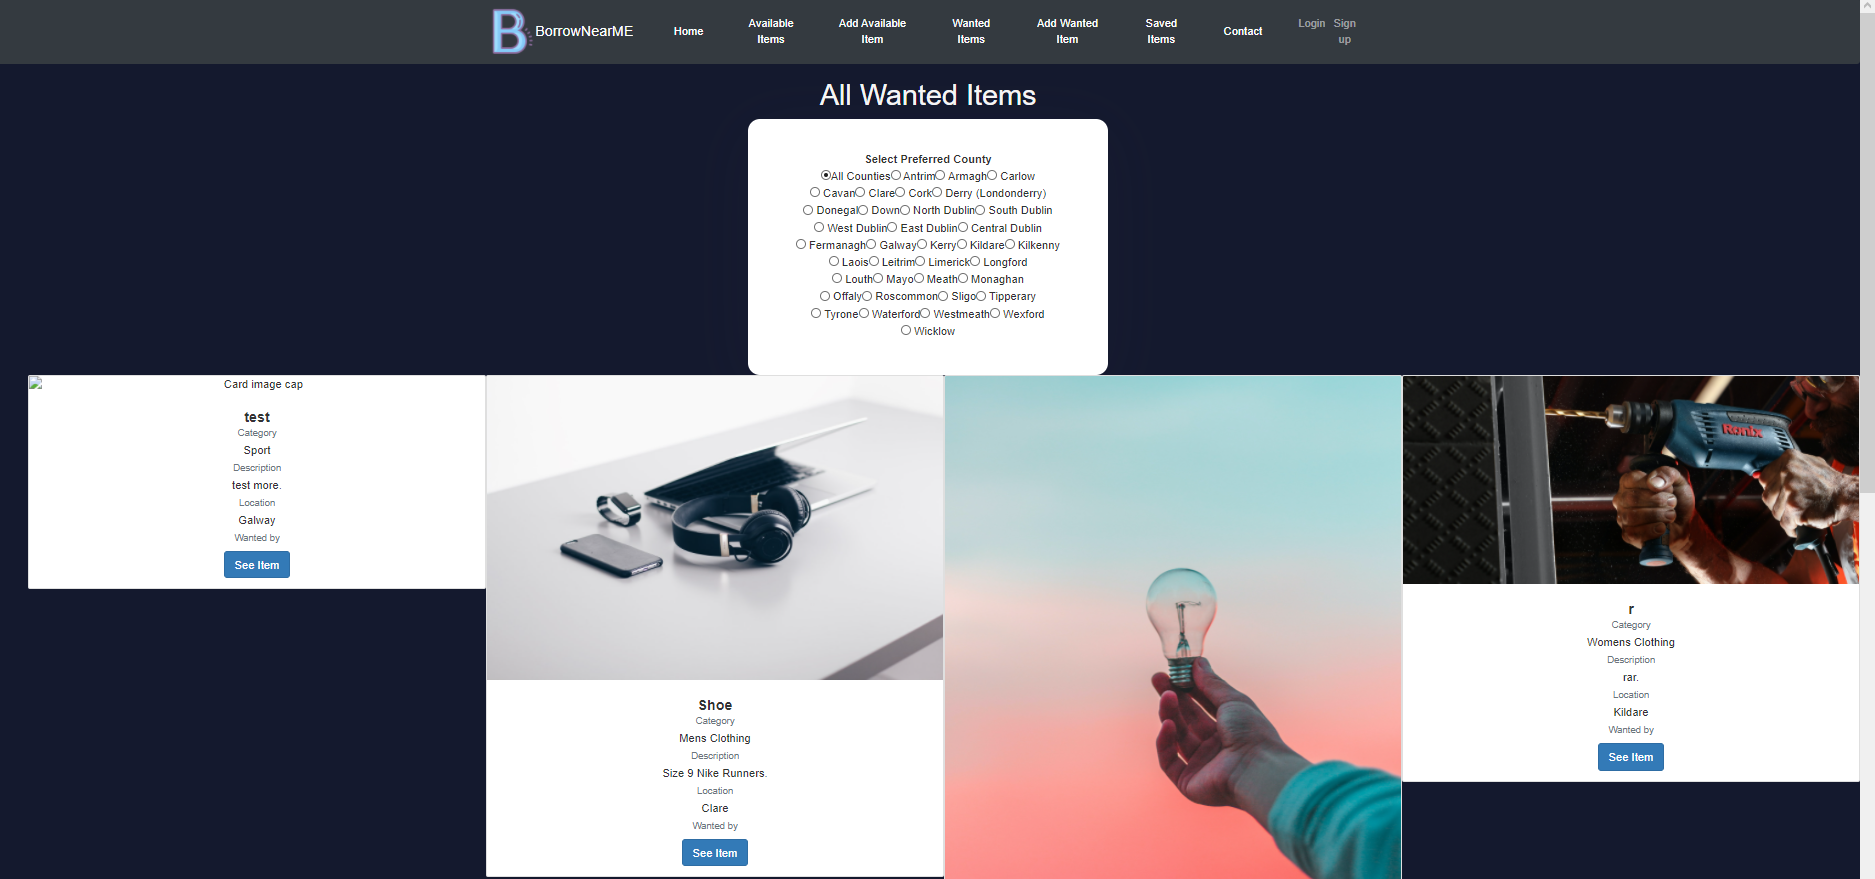
\includegraphics[width = \textwidth]{img/fe_wanteditems.PNG}
\caption{View Wanted Items page}
\label{WantedItems}
\end{figure}

\begin{figure}[h]
\renewcommand\thefigure{4.4}
\centering
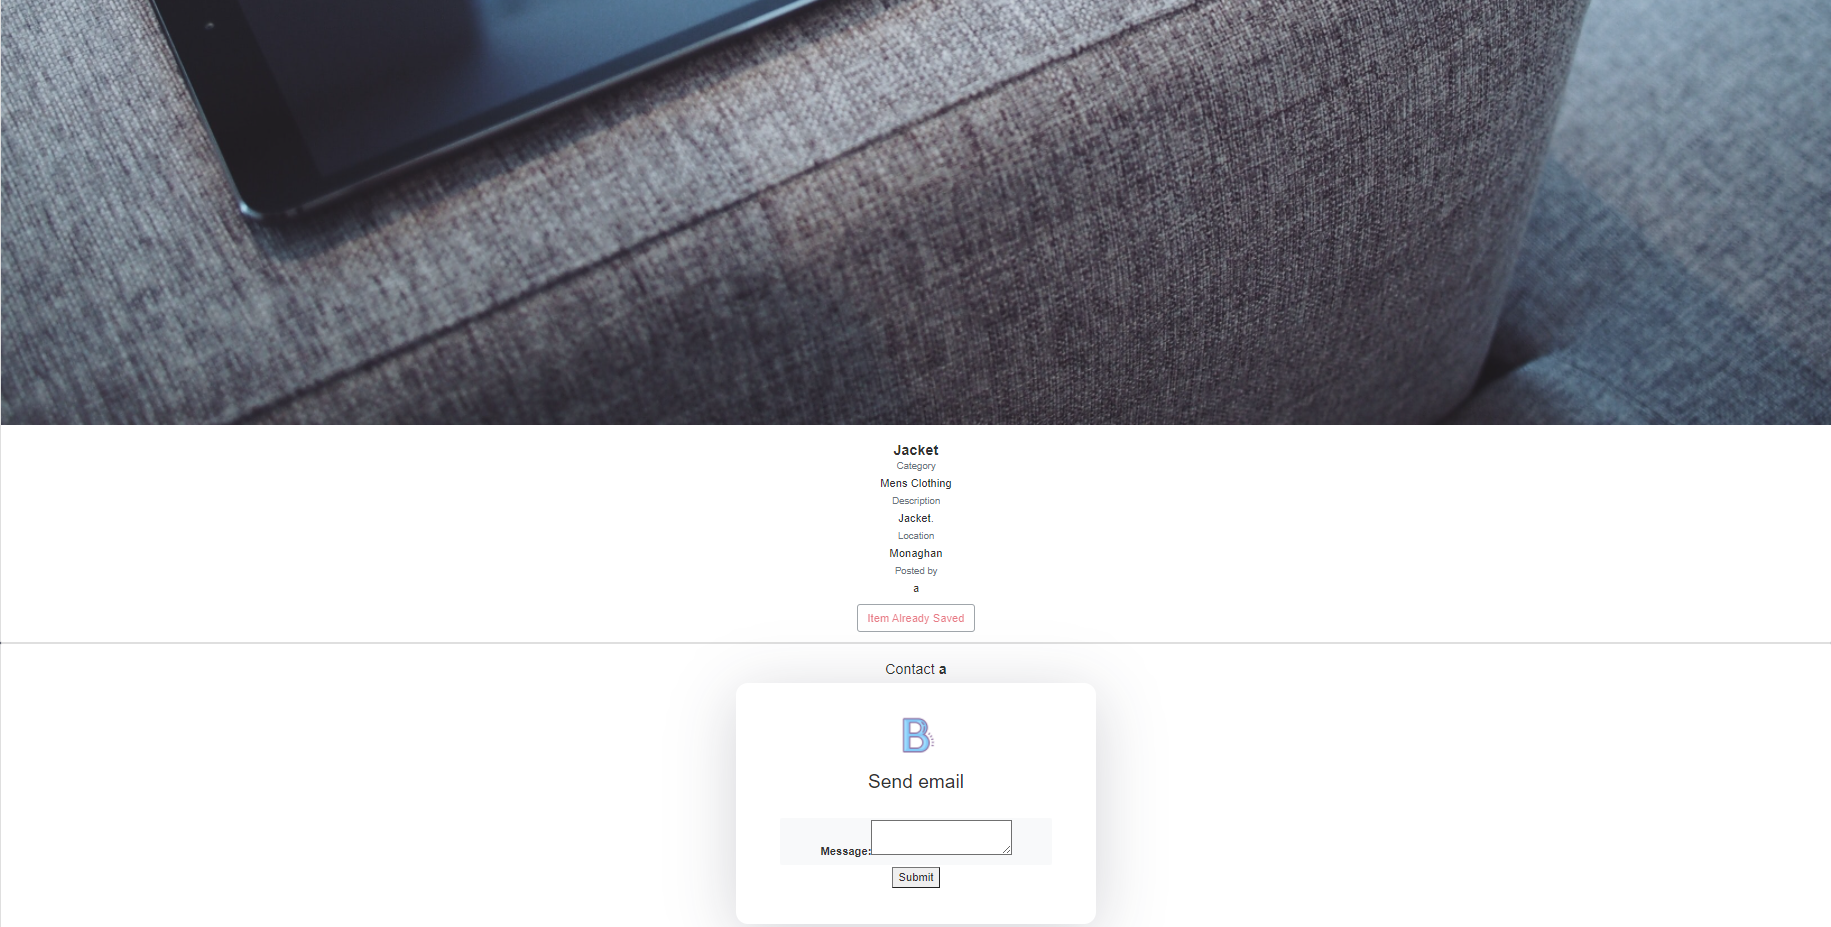
\includegraphics[width = \textwidth]{img/fe_itemcontact.PNG}
\caption{Contacting users}
\label{Contact}
\end{figure}
\newpage

\subsubsection{Add Items}
Users can add items for trade and wanted items to the database which is used to display the items. The user must be logged in to use the add item pages and once they're their they must input a name, category, description and location. They must also choose an image to represent the item.

\begin{figure}[h]
\renewcommand\thefigure{4.5}
\centering
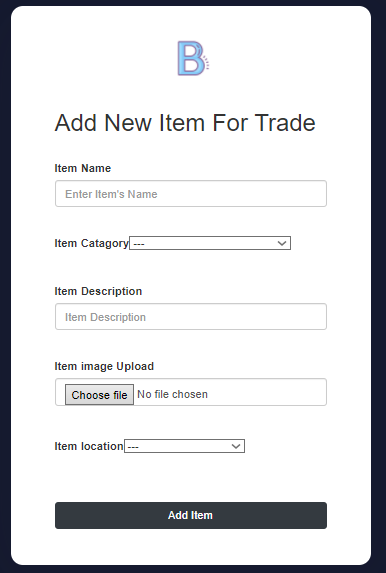
\includegraphics[scale=.6]{img/fe_additem.PNG}
\caption{Adding items}
\label{AddItem}
\end{figure}

\subsubsection{My Account}
The account page has 3 options for users:
\begin{enumerate}
  \item My Available Items
  \item My Wanted Items
  \item My Saved Items
\end{enumerate}
By selecting "My Available Items" or "My Wanted Items", the user will be brought to a page that displays the available/wanted items which they have posted themselves. From here, they are able to delete these items or edit the details of the items by clicking the designated buttons.

\begin{figure}[h]
\renewcommand\thefigure{4.6}
\centering
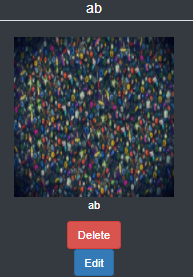
\includegraphics[scale=.6]{img/fe_editdelete.PNG}
\caption{Available Item in "My Available Items"}
\label{AvailableItem}
\end{figure}

They can also view the items belonging to other users which they have saved. The user is able to view information about any of these saved items by simply clicking on them. 

\subsubsection{Contact form}
The contact form is a simple page which contains a small box which prompts the user to input their name, email and message. Once they have filled out the form, they can send it to the 'barter4tradenc' email address by clicking on the 'Submit' button.

\begin{figure}[h]
\renewcommand\thefigure{4.7}
\centering
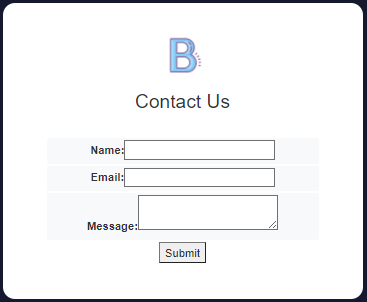
\includegraphics[scale=.6]{img/fe_contact.PNG}
\caption{"Contact Form"}
\label{ContactForm}
\end{figure}

\subsection{Back End}

\subsubsection{Starting up}
There's no prerequisites to setting up a Spring Boot Application other than having a version of Java installed (We would recommend 8 or above) and an Integrated Development Environment (We would recommend IntelliJ). Inside your IDE, create a new Spring web tool to create the Spring Boot project. This will automatically create most of the files you need for your Spring Boot Application to work. \par
The next step is to open the pom.XML file. This file should be located in the main directory of your project, not within a package. Here is the location of all of the dependencies that the Spring Boot Application will install. The one needed for Mongo and the JWT authentication are as follows: \par
\begin{minted}[]{java}
<dependency>
  <groupId>org.springframework.boot</groupId>
  <artifactId>spring-boot-starter-data-mongodb</artifactId>
</dependency>
<dependency>
  <groupId>org.springframework.boot</groupId>
  <artifactId>spring-boot-starter-security</artifactId>
</dependency>
<dependency>
  <groupId>org.springframework.boot</groupId>
  <artifactId>spring-boot-starter-web</artifactId>
</dependency>
<dependency>
  <groupId>io.jsonwebtoken</groupId>
  <artifactId>jjwt</artifactId>
  <version>0.9.1</version>
</dependency>
\end{minted}

\subsubsection{Sign up}
From the beginning of the first semester, the main goal of the project was to achieve a working sign up and login. Naturally it made more sense to begin with a Sign up functionality, to be able to send data to our database through our API. To explain how this will work in lament terms:
\begin{itemize}
    \item POST: an API POST request will be sent to the Spring Boot API.
    \item Check: The Server will check is the current user exists in the database
    \item Return: A Return message of either "Registered successfully" or "Username is already taken" will be sent back.
\end{itemize}
\par The signup request is a POST request. Firstly the function checks id the signUpRequest's username is already in use, and then checks if the email is in use. If neither of these are in use it moves to the next step, creating a user: \par
\begin{minted}[]{java}
 User user = new User(signUpRequest.getUsername(),
                signUpRequest.getEmail(),
                encoder.encode(signUpRequest.getPassword()));
        Set<String> strRoles = signUpRequest.getRoles();
        Set<Role> roles = new HashSet<>();
\end{minted}
\par This code sets the username, the email, password and the role(user by default) to local variables for now. The code then executes some checks to ensure that the role sent with the signup request exist, and then finally we save the new user to a MongoDB userRepository: \par
\begin{minted}{java}
  userRepository.save(user);
  return ResponseEntity.ok(new MessageResponse("User registered successfully!"));
\end{minted}

\subsubsection{Login}
After we tested our new API request, by using Postman and Robo 3T, the next step was to make a login feature, to ensure we could retrieve data from our MongoDB Database as well. This API also has numerous steps that we will explain below: \par
\begin{itemize}
    \item POST: The username and the password are sent to the Spring Boot API.
    \item Authenticate: The username and password are checked if accurate within the database and sends back a JWT string with a secret.
    \item Return: The API sends back a JWT response to the requester if the username and password are correct.
\end{itemize}
The signin is also a POST request, as the username and password are getting sent to the API. To start, the username and the password are sent to an instance of the AuthenticationManager class. If the principal of the input authentication is valid and verified, AuthenticationManager#authenticate returns an Authentication instance with the authenticated flag set to true. Otherwise, if the principal is not valid, it will throw an AuthenticationException. For the last case, it returns null if it can't decide \cite{Baeldung}. \par
\begin{minted}{java}
 Authentication authentication = authenticationManager.authenticate(
        new UsernamePasswordAuthenticationToken(loginRequest.getUsername(),
        loginRequest.getPassword())); 
\end{minted}
\par After this the method generates a JWTToken. The method checks the user's role and grants them authority dependant on this. We don't utilize this as all users of the website are simply "User" as oppose to giving some admin and moderator. We didn't need this but its a built in function in JWT, so it doesn't cause any overloading or unnecessary code, it could be implemented at a later date. Lastly the method returns a response with the JWT, the user id, username and the email.\par
\begin{minted}{java}
 return ResponseEntity.ok(new JwtResponse(jwt,
                userDetails.getId(),
                userDetails.getUsername(),
                userDetails.getEmail(),
                roles));
\end{minted}

\subsubsection{Add Item}
We had completed the development of the  Sign up and the Login component before the December presentation in the first semester. We each took a few weeks off after that to allow for holidays, work on other individual projects and for some personal time. When we began development again in late January. The main focus of the Back End development was to allow the users of the website the ability to add items to the database and to be able to retrieve this information. The classes associated to this are as follows: \par
\begin{itemize}
    \item Model: This class is a document collection, that comprises of the variables needed for the item (name, category, location etc), the getters and setters for variables and a constructor.
    \item Repository: This class is an interface that comprises of two lists, a list of the items sorted by their title(name) and sorted by if they're published or not.
    \item Controller: This class is where all of the MongoDB database API calls are declared.
\end{itemize}
\par The Model has a toString method that we use to set the variables in a String format to allow it to be stored in the MongoDB database. This is essential as with MongoDB being a Document based database, the information has to be in a JSON format for it to be saved and stored correctly. \par
\begin{minted}{java}
@Override
    public String toString() {
        return "Tutorial [id=" + id + ", title=" + title + 
        ", desc=" + description + ", published=" + published +
        ", category=" + category+ ", username=" + username+ 
        ", email=" + email +", imagerurl=" + imageurl+ 
        ", location=" + location+ "]";
    }
\end{minted}
The Repository is essential for the storage of the items in the database. Its also thanks to this interface, that allows us to search and retrieve specific items from the database. \par
\begin{minted}{java}
List<Tutorial> findByTitleContaining(String title);
\end{minted}
The main class in the addition of items is the controller. This Class allows for the API calls, similar to the AuthController in the signup-login components. We have a function that calls all of the items from the database, this is used for the Available items page in the front end. There are also functions for the addition and the update of items within the database. This is also where the delete function is declared.
\begin{minted}{java}
@GetMapping("/tutorials")
    public ResponseEntity<List<Tutorial>> getAllTutorials(@RequestParam
    (required = false) String title) {
        try {
            List<Tutorial> tutorials = new ArrayList<Tutorial>();
            if (title == null)
                tutorialRepository.findAll().forEach(tutorials::add);
            else
                tutorialRepository.findByTitleContaining(title).forEach
                (tutorials::add);
            if (tutorials.isEmpty()) {
                return new ResponseEntity<>(HttpStatus.NO_CONTENT);
            }
            return new ResponseEntity<>(tutorials, HttpStatus.OK);
        } catch (Exception e) {
          return new ResponseEntity<>(null, HttpStatus.INTERNAL_SERVER_ERROR);
        }
    }
\end{minted}
The code from these parts of the Back End Environment were adapted from this cite \cite{zKoder}.

\subsubsection{Wanted Item}
When the development of the add items was complete, the next objective we turned our focus to was the Wanted Items page. This is for when a user is looking to buy or purchase an item, they can post to this page to advertise their want for this item. \par
The overall design of the Wanted Item's Back End classes are similar to the Add Items. As both items are structurally the same (the need for item name, category, location etc), we felt this was the best method of moving along with its development. Due to this, the Wanted Items is functionally the same as Add Items, therefore we wont repeat ourselves by showing the model, controller and repository for these classes, as the code is very similar to the code explained above in the Add Item section. \par

\subsubsection{Saved Item}
The development of the Wanted Item was completed in early March. After this was a lull in the Back End environment as we were working on other modules and Cathal was attempting to get the AWS for the website functional. In early April we created the Saved Items function. This was to allow users to add items from the available items, to another page of their own displaying the items they intended on purchasing or trading for in the future. \par
The structure behind this is similar to the Add Item and the Wanted Item. They contain a Model, a Controller and a Repository that work very similarly to the classes in the other components mentioned above. There are small difference however, as we only needed to store an ID, a username and a title in the Saved Item. We use these variables to search through the available items, and to display only the items with the same ID as the ones stored in this repository. This is done through a method in the controllers: \par
\begin{minted}{java}
@GetMapping("/wanted/{id}")
    public ResponseEntity<WantedItem> getWantedItemById(@PathVariable("id")
    String id) {
     Optional<WantedItem> WantedItemData = wantedItemRepository.findById(id);
        if (WantedItemData.isPresent()) {
            return new ResponseEntity<>(WantedItemData.get(), HttpStatus.OK);
        } else {
            return new ResponseEntity<>(HttpStatus.NOT_FOUND);
        }
    }
\end{minted}

\section{How they work together}
This section outlines how we intertwined the React with Spring Boot and MongoDB. This was mainly done through pair programming as Cathal understood all of the back end elements, while Nathan understood all of the Front End elements. Upon completion of the back end elements, we scheduled a meeting between us whereby Cathal showed how all of the back end elements worked through the use of discord, robo, postman and docker. This methodology allowed us both to gain a better understanding on how each environment of the project worked. \par
The first task was installing Axios, which is a Node.js library that allows us to make HTTP requests to external sources. Axios was the best choice as we had both used it before as part of a 3rd Year project and it is not too difficult to configure, offers a lot of good documentation and a wide community due to its popularity and offers really good error handling that makes debugging problems a lot easier. \par
When a user enters their details to sign up and clicks submit, the username, email and password that they input gets gets sent to the server via a POST method, which will only be sent successfully if the details entered are not already saved.
\par
\begin{minted}{js}
axios.post('api/auth/signup', data).then(
            res => {
                localStorage.setItem('token', data.token);
                localStorage.setItem('user', data.username);
                localStorage.setItem('email', res.data.email);
                this.setState({ loggedIn: true });
                window.location.reload(false);
            }
        ).catch(
            err => {
                console.log(err);
            }
        )
\end{minted}
The reason why we set the state of loggedIn to true and reload the window is because the first thing done inside the render of the classes which are used to provide the database with data is checking if we are in a loggedIn state and returning to the home page if we are. This is done so that the user knows that their item has been posted successfully and it prevents users from needlessly spamming registrations. Its done particularly in the sign up page so that the navigation bar's state is changed correctly when the user returns to the homepage. \par
The other HTTP methods which we use to send and retrieve data are 'put' and 'get' methods.
\begin{minted}{js}
state = {
        items: []
    }
    componentDidMount() {
        axios.get(`api/test/tutorials`)
            .then(res => {
                const items = res.data;
                this.setState({ items });
            })
    }
\end{minted}
In the above code, we perform a http get request to return the information about all available items from 'http://localhost:8081/api/test/tutorials'. With this data, we are able to show the user all of the current available items by displaying a card containing all of the item details, for every item that is returned.
\begin{minted}{js}
axios.post('api/test/tutorials', data).then(
            res => {
                console.log(res);
                this.setState({
                    itemAdded: true
                });
            }
\end{minted}
Above, an array of items called 'data' which contains the details of the item to be added is sent to the database via an axios 'post' method. Once again, the change in state is there so that the user is returned to the homepage after the item has been added to the database. The most complicated part of this was getting the image to store to the database and to solve this the image first had to be converted to base64 as the database is designed to deal with textual data and base64 is the best way to store an image in text form. 
\begin{minted}{js}
getBase64(file, cb) {
        let reader = new FileReader();
        reader.readAsDataURL(file);
        reader.onload = function () {
            cb(reader.result)
        };
        reader.onerror = function (error) {
            console.log('Error: ', error);
        };
    }
    handleImageChange(e) {
        alert(e.target.files[0]);
        this.getBase64(e.target.files[0], (base64) => {
            this.setState({ Base64Image: base64 });
            this.image = base64;
        })
    }
\end{minted}
To edit items, we first get the data of a certain item has stored by performing a HTTP get request that returns the data of a chosen item. This data is then used to popular the placeholders of the item details, which can be changed or left the same to the users desire. Once the user is happy with the changes and they click the confirmation button, the new data will be sent to the same url using a put method. The put method replaces the data that is currently stored in the database rather than overwriting it which is perfect for editing items.
\begin{minted}{js}
axios.get(`api/test/tutorials` + this.props.match.params.id)
      .then((res) => {
      title: res.data.title,
      category: res.data.category,
      etc.....
}
onSubmit(){
    axios.put(`api/test/tutorials/` + this.state.id, newItem)
          .then((y) => {
            console.log(y);
        })
        .catch((err) => {
            console.log(err)
        });
}
\end{minted}
The final HTTP method which is used to connect the Front end with the back end was the delete method, which is only used when a user deletes one of their available or wanted items.
\begin{minted}{js}
// replace (dollarsign) with a dollar symbol
deleteItem(id, e) {
        axios.delete(`api/test/wanted/(dollarsign){id}`)
            .then(res => {
                console.log(res.data);
                window.location.reload(false);
            })
            .catch((err) => {
                console.log(err);
            })
    }
\end{minted}
\chapter{System Evaluation}
This part of the dissertation will be dedicated to the testing and evaluation of the project. We will compare our objectives of the dissertation to the functionality of the application. This section will also cover the comparison of the timeline that we set out to follow in the development process and the timeline in which those objectives were reached. We will then move onto the testing process and conclude this chapter by listing our limitations of the project.\par

\subsection{Objectives}
To begin the System Evaluation we will begin by reiterating over our objectives set in the introduction. The main functionality we wanted to achieve was:
\begin{itemize}
    \item Users can register and browse items
    \item Users can select to borrow items from other users
    \item Users can view the owners of items and contact them
    \item Users can add items to a wish list
\end{itemize}
\par Upon our evaluation of the objectives listed above, we feel that we did achieve them all. Users can register through the sign up option on the NavBar. Users can browse the available items, whether they are currently signed in or not, allowing completion of objective one. These available items are able to be published by anyone, and can be viewed by everyone, completing our second objective. The third objective listed above has also been completed once the user has been logged in, where they can send an email to the owner of the item. Lastly, the users can add items to their wish list page through the SavedItems component. With this recap of our objectives and the functionality of the application, we believe that all of the tasks we lined out in our objective section have been achieved completely. \par

\subsection{Timeline and Scope}
\begin{figure}[h]
\renewcommand\thefigure{5.1}
\centering
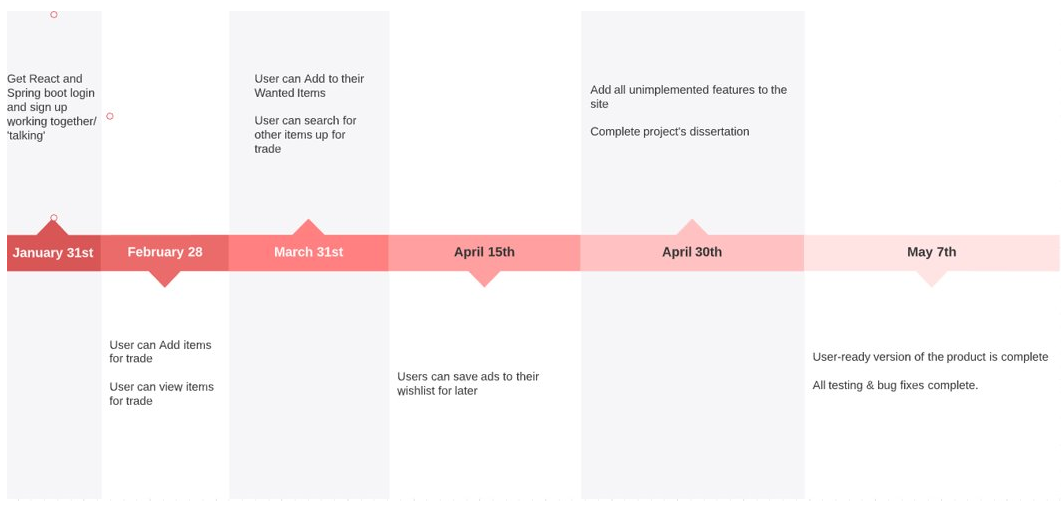
\includegraphics[scale=0.4]{img/timeline.png}
\caption{"Project Timeline"}
\label{Timeline}
\end{figure}

This graph lays out the timeline that we set for ourselves after the completion of the 1st semester. As we lost Anton just before the Christmas period, this led us to have to reevaluate our entire process and the scope of the project. 
\begin{itemize}
    \item January 31st - This date was the goal to achieve the login and the sign up functioning in the react Front End i.e. making it possible to sign up and login with the spring boot through the app. This goal was achieved on this date exactly.
    \item February 28th - This was the date in which we wanted it to be possible to add and view the items added to the database. This goal was achieved before this date, on the 16th of February leaving us ahead of our scope.
    \item March 31st - By this date we had planned on having the wanted items functionality working. This goal was reached on the 4th of March, almost a month ahead of what we had planned.
    \item April 15th - The goal for this date was to have the users being able to save items to their wish list. This goal was achieved on the 13th of April.
    \item April 30th - We had aimed to have all features of the website functioning and to have the dissertation completed by this deadline. Due to circumstances relating to other modules, this goal was not reached. By this date we had achieved all functionality, other than contacting other users and the dissertation was not complete.
    \item May 7th - This date was dedicated to having all testing and bug fixes implemented by. By this date, as the deadline for the project had changed, we still hadn't completed the dissertation. most bug fixes had been achieved, but not completely.
\end{itemize}

\subsubsection{Evaluating our Timeline}
When the development of our project had begun properly, we made good use of the timeline and achieving the deadlines that we had set for ourselves. But as the timeline moved on, and other module's assignment dates grew closer, we started to miss our deadlines. There were also personal reasons behind such complications, mostly due to COVID-19 and our own mental health. These goals were still reached, none the less, but just late. We are still very pleased with our completion of our objectives, despite the missing of goals, when we consider that our three man project became a two man project.

\subsection{Testing}
Our testing was executed as the goals that we had set for ourselves were achieved. We did this to ensure that we were happy with each individual component of the application before we started the development of another. As we used an Iterative and Incremental development process, we commenced the testing of these components as soon as we felt that we had achieved a new iteration in the design.\par
This was done through white box testing, where the tester has knowledge as to the components and the functionality of the software in question. This was essential in our development as it allowed us to confirm that our programs were executing as designed. This method however, led to some of our bugs being discovered later in the development, where if we had implement black box testing, these may have been discovered earlier in the development. \par 
When we were pair programming, as soon as a new commit was made by one of us to either the Front End or the Back End, we immediately pulled the new commit and tested the new function to ensure that they were working on both machines. This method of testing allowed us to always have a working version of the application on GitHub and to also allow us to confirm that the code could be cloned and work on another station.\par
We conclude that this endeavor resulted in a more robust framework overall, and we were able to move on with the project after completing these tests. We are confident with the method that we used to test, and to confirm our code was executing properly, that the system we have designed now is robust due to its ability to cope with errors on compile time.

\subsection{Limitations}
There were many complications that were met along the way of this project. They range vastly in terms of small issues with JSON data formatting, all the way to having to change the structure of the design completely. The first issue we will be discussing is the change of Back End environment that we made in the 1st semester. \par
As we already explained, we had originally planned on using a flask application coded through Python for the Back End environment. This was planned from the very beginning of the development cycle. Cathal and Anton were the ones in charge of this implementation. They researched into Flask together and attempted to get a functioning sign up and login in working in Flask. \par
In mid October however, we were required to install Anaconda onto our machines for another module, Emerging Technology. This module was a Python focused module and used Anaconda to execute most of the commands. When Anaconda was installed on our machines however, it blocked some of the Python functions on our drives, namely where the .py executable is called from. Since we couldn't uninstall Anaconda as we needed it for the module, we opted to change the Back End Environment entirely and switched to Spring Boot in Java. Other than this change in the Back End environment, there weren't many other limitations we came across. \par
When it came to the MongoDB Database we chose for storing our information, there were very few limitations to speak of. The main hurdle we encountered was that everything that was to be stored in the MongoDB Database must be first declared as a document and must be in a JSON format to be stored properly.
\chapter{Conclusion}
We are both extremely happy with the final result of our hard months of work for this Final Year Project. It was both challenging and rewarding in its own way. We enjoyed our own free reign to make requirements and the ability to challenge them in any method we found fit to. We found that choosing our own technologies and having to overcome their short ends and their limitations resulted in a learning curve that couldn't have been accomplished by any other means. After seven months of designing, researching, planning, development and deployment we are happy to confirm that we have completed the project. \par
To reevaluate again, the goal of our project was to develop a full stack CRUD application developed for trade and exchange of items between multiple users. The Back End data storage was wrote in Java with a Spring Boot framework, and the Front End was wrote in JavaScript as a React application. We will now re-summarise our objectives of this project. \par

\section{Objectives}
The first objective of the project was to ensure that a new user to the website could firstly access the website, could then register and sign in with the credentials entered in the registry, and lastly could then browse and view items that are available for trade on the website. This was achieved as early as mid-February. We were extremely pleased with this project so early in the development process. \par
The next object we will bring to light is to allow users to select the items from other users. This was mostly implemented in early April, as Nathan added an entirely new page that would display the details associated with the item the user was to click on. This was implemented late in the development process, this was due to it not being a major priority of the project at the time. \par
The objective after this was for users to be able to view the owner of the item and to have the ability to contact them. This was the most recent objective to be reached, as there were many complications with the server communicating with our react application. We pondered on how implement this function for some time, without exposing any private information of the users of the application. This was a focus of ours to ensure that we get their private data secure. We finally opted to have the gmail we created for this project, to send an automated email to the owner with the interested buyers email. The follow up of this contact is up to the owner entirely, relieving us of any legal issues. \par
Lastly, the objective for users to be able to add items to their wish list. We managed to accomplish this objective earlier than we anticipated. We simply saved the id of an item to a new container containing a username and an id. This allowed us to retrieve the data quickly and efficiently with little complication. \par

\section{Findings from the System Evaluation}
When we completed the System Evaluation section of the dissertation we were surprised to find how many objectives we completed with ease. The biggest surprise of these findings was how well we kept to the scope. We managed to pull ahead of the original deadlines we had set out in early January. We didn't make the later deadlines as we ran into numerous complications with getting users to communicate and with deploying the application to AWS. \par
We are overjoyed to be able to claim that we believe we have achieved all of the objectives we set out when we began the project. These are:
\begin{itemize}
    \item To create a CRUD application in an environment we didn't have much experience in.
    \item To work with new technologies and to improve our understandings of said technologies.
    \item To challenge ourselves to build a full stack application and to deploy it
    \item Improving our team working abilities and to simulate a work style environment.
\end{itemize}

\section{Future Improvement}
After analyzing our progress thus far, and evaluating the elements of our development process that has led us to the current version of the application we have found a number of areas that we could've improved on and changed entirely.\par
To start Nathan would've liked to have add more categories for the users to choose from to improve user satisfaction and to make the application even more diverse. There are a lot more possible item categories and placing the majority of items into the miscellaneous category doesn't really provide the adequate user experience. More possible item categories makes it easier for the user to browse items which interest them more and even locate specific items. \par
Cathal feels that the Back End could've also done with some key improvements. The retrieval of user info requires a Bearer Key for the API call to be authorized, this possibly could've been edited to allow the front end to access the information without saving it to local storage. \par
We both feel that if we had more time, that a chat feature of the application could've been implemented instead of an automated email. The bug fixes and the AWS took longer to fix than we had envisioned and we ran out of time to implement this. \par
Another feature that we would've like to have added would have been a search feature. Technically, the items can be searched for a particular id, but if we had more time, we would have done so using the title(name) of the item as well, allowing for a search bar feature. \par
To conclude we are both still very happy with the outcome of this project and feel that our skills have really developed from the complications and difficulties we encountered. We are very proud to announce that despite loosing a member of our team after our planning and designing of the application, that we didn't loose and features or functionality that we had set out on doing before hand.

\section{Thanks}
We would like to thank our lecturer and supervisor Martin Kenirons again for all the help and support he provided us with. His guidance and counsel was a vital contribution to us achieving our goals.
